\documentclass[10pt,oneside,a4paper,onecolumn,titlepage,draft]{lancsthesis}
% =============================================================================

\usepackage{lancsthesis}    % Book format, local copy
\usepackage{swLaTeXTools}   % Custom additions and commands

% UTF-encoded input files
\usepackage[utf8]{inputenc}

% Allow insertion of outline
\usepackage{pdfpages}

% Change the way footnotes are numbered.
\usepackage{chngcntr}
\counterwithout{footnote}{chapter}

% \text and more in math mode
\usepackage{amsmath}

% Merging table cells.
\usepackage{multirow}
% Remove me after drafting
\usepackage{ifdraft}

% Code Listings
\usepackage{listings}
\lstset{breaklines=true}
\lstset{numbers=left}
\lstset{captionpos=b}
\lstset{extendedchars=true}

% Font: URW Palladio (Palatino clone)
\usepackage{pxfonts}
\usepackage[T1]{fontenc}

% Line spacing needed for lancsthesis
\usepackage{setspace}
\linespread{1.45}    % double spacing is 1.6, half is 1.3
% \onehalfspacing
% \doublespacing

% Ability to include PDFs
\usepackage{pdfpages}

% configure graphics
\setkeys{Gin}{draft=false}  % Graphics show in draft mode
\usepackage{graphicx}
\graphicspath{ {./images/} }
\DeclareGraphicsExtensions{.pdf,.png,.jpg,.eps}

% Rotation of some figures and tables
\usepackage{rotating}

% Multi-page tables
% Used in tex/persona/results.tex only, commented out there.
% \usepackage{longtable}

% Two-column spanned tables
% \usepackage{supertabular}

% Two column blocks
% \usepackage{multicol}

% Subliminal text position hints
% Requires PdfTeX, XeTeX or LuaTeX
\usepackage{microtype}

% Restrictions on figure movement
\usepackage{placeins}

% hyperref
\usepackage{hyperref}
\hypersetup{
    pagebackref=true,
    final=true,     % Show even when doc is in draft mode
    hidelinks=true,
    unicode=true,   % Enable the 21st century
    pdfborder={0,0,0,[]},
    pdfauthor={Stephen Wattam},
    linkbordercolor={0 0 0},
    citebordercolor={0 0 0},
    urlbordercolor={0 0 0},
    urlcolor=blue,
    filecolor=black,
    citecolor=blue,
    linkcolor=black,
    colorlinks=true,
    bookmarks=true
}

% PDF bookmarks
% \usepackage{bookmark}


% ------------------------------------------------------------------------------
%  Drafting 
% ------------------------------------------------------------------------------
%
% Watermark if in draft mode
\ifdraft{
    \usepackage{draftwatermark}
    \SetWatermarkScale{1.5}
    \SetWatermarkLightness{0.95}
}{}

% Page layout (margins)
\ifdraft{
    % inline layout
    \usepackage[left=38mm,top=25mm,right=38mm,bottom=25mm]{geometry}
}{ % else
    % book layout (asymmetric)
    \usepackage[left=38mm,top=25mm,right=25mm,bottom=25mm]{geometry}
}

\ifdraft {
    \usepackage{todonotes}
    \newcommand{\td}[1]{\todo[fancyline,size=\tiny,color=yellow!20]{#1}}
    \newcommand{\til}[1]{\todo[inline,size=\small,color=yellow!20]{#1}}
}
% ------------------------------------------------------------------------------





% =============================================================================
%  Begin document
% =============================================================================
\begin{document}
\frontmatter
% \thispagestyle{empty}



% =============================================================================
%  Title Page
% =============================================================================
%% TODO: port this to the lancsthesis.cls style as \title
\begin{center}
\begin{tabular}{c}
\vspace{2in}\\
\begin{minipage}{5in}
\begin{center}
{\bf \huge 

	
Big Scary Thesis Title:\\


Powered by Tea and delusion\\
%{\small `tea' is capitalised because it fucking rocks.}
% TODO

}
\vspace{2in}


{\bf \Large Stephen Wattam}

\vspace{2in}


Submitted for the degree of Doctor of Philosophy\\
at Lancaster University, \\
January 1901.
% TODO

\end{center}
\end{minipage}
\end{tabular}
\end{center}
\newpage






% =============================================================================
%  Introductory items
% =============================================================================
\chapter*{Abstract}
Current efforts in corpus linguistics and natural language processing make heavy use of corpora---large language samples that are intended to describe a wide population of language users.

% Historically these items have had their utility abrogated by a number of economic, social and practical limitations.

The first modern corpora were manually constructed, transcribed from published texts and other non-digital sources into a machine-readable format.  In part due to their hard-won nature, larger corpora have become widely shared and re-used: this has significant benefits for the scientific community, yet also leads to a stagnation of sampling methods and designs.

The rise of Web as Corpus (WaC), and the use of computers to author documents, has provided us with the tools needed to build corpora automatically, or with little supervision.  
This offers an avenue to re-examine and, in places, exceed the limitations of conventional corpus sampling methods.  
Even so, many corpora are compared against conventional ones due to their status as a de-facto gold standard of representativeness.  Such practices place undue trust in aging sample designs and the expert opinion therein.

%---

In this thesis I argue for the development of new sampling procedures guided less by concepts of linguistic balance and more by statistical sampling theory.
This is done by presenting three different areas of potential study, along with exploratory results and publicly-available tools and methods that allow for further investigation.

The first of these is an examination of temporal bias in sampling online.  I present a preliminary investigation demonstrating the prevalence of such effects, before describing a tool designed to reveal linguistic change over time at a resolution not possible with current software.

Secondly, the sample design of larger general-purpose corpora is inverted in order to relate it to an individual's experience of language.  This takes the form of a census sample of language for a single subject, taken using semi-automated methods, and illustrates how poorly suited some aspects of general-purpose corpora are for questions about individual language use.

Finally, a method is presented and evaluated that is able to describe arbitrary sample designs in quantitiative terms, and use this description to automatically construct, augment, or repair corpora using the web.  This method uses bootstrapping to apply current sampling theory to linguistic research questions, in order to better align the scientific notion of representativeness with the process of retrieving data.

%I apply these novel methods to the problem of improving WaC samples (whilst avoiding their novel pitfalls), and present ways in which the whole scientific process of corpus comparison, dissemination and replicability may be assessed---itself something that demands an alternative view of corpus goals.I go on to present tools that make these tasks easy to apply in a scientific context, in order to construct usable and practical web-derived corpora.



%\pagebreak

\chapter*{Acknowledgements}

This thesis could not have been completed without the support of many people.  Foremost  amongst these must be my supervisors, Paul Rayson and Damon Berridge.  Their direction and encouragement was often the only thing keeping me in the office.

Secondly, my friends, particularly Carl Ellis and John Hardy, have been instrumental in honing my approach to work and life.% TODO: more.

Finally, I wish to thank my parents.  It is doubtless my mother's lesson to question the world that has lead me into research, and my father's work ethic (however diluted during inheritance) that has carried me this far.

\begin{center}
Thank you all.
\end{center}




%\pagebreak

\chapter*{Declaration}
% The material presented in this thesis is the result of work by...
The material presented in this thesis is the result of original research by the named author, Stephen Wattam, under the supervision of Dr. Paul Rayson \& Prof. Damon Berridge, carried out in collaboration between Maths and Stats and the School of Computing and Communications, Lancaster University.

This work was funded by the Economic and Social Research Council.  Part of this thesis are based upon prior publications by the author, listed below---all other sources, if quoted, are attributed accordingly in the body of the text.

\begin{itemize}
    \item CL'11 ref.
    \item WaC8 ref.
    \item CL'13 ref.
\end{itemize}

% space for signature
\vspace{1in}
Mr Stephen Wattam \dotfill


% space for supervisor's signature
\vspace{0.5in}
Dr Paul Rayson \dotfill






%% space for supervisor's signature
%\vspace{1in}
%\dotfill DB 

%\pagebreak

% Auxiliary introductory things
\tableofcontents
\listoffigures
\listoftables
\clearpage



% =============================================================================
%  Start of Actual Content
% =============================================================================
\mainmatter


\chapter{Introduction}
\label{sec:introduction}


We have seen in previous chapters (\td{which}) a number of scientific and practical issues that affect current corpus collection methods.

This chapter details the design and implementation of a method for performing number of common corpus building workflows.  These workflows are designed both as a continuation of the methods detailed in Chapter~\td{chapter 4} and as part of work with existing corpora, and represent areas of scientific importance in corpus studies.




The chapter begins in Section~\ref{sec:rebuilding:rationale} with an outline of the workflows involved, detailing the rationale behind each, and the value that formalising the process may yield.  Immediately following is an outline of the design of the method, specifying the processes involved and comparing them both to existing procedures and to the original workflows.

Section~\ref{sec:rebuilding:method} describes the mechanisms used to implement these designs, and covers the architecture of the software used to test the method.  It discusses the algorithms used, as well as the variables selected for the test system and the strengths and weaknesses of these as a mechanism for evaluating the method described earlier.  This section then specifies the technical details of the implementation, and provides details on the approximation and optimisation methods used.  

Finally, the conclusion relates the design and implementation of the method back to the aims detailed in \td{ref chapter 2}, drawing comparisons again to the capabilities of other existing systems.




\chapter{Review of Literature}
\label{sec:litreview}
% ---------------------------------------------------------------------------------------------------------------------

\til{Intro to use of corpora --- basically what people do with them [note, not what they are, that comes later], what they contain (roughly) and special/general purpose.  See this as an intro for non-linguists and some signposting}


% ---------------------------------------------------------------------------------------------------------------------
\section{Corpora and Corpus Linguistics}
\label{sec:litreview-corpora}


The field of linguistics is one concerned with description and formailisation of a particularly ethereal social concept.  The paucity of philosophical agreement upon the nature of language has led to many different approaches being taken through the years, many of which have accomplished great things in advancing our capacity to reason about, and derive conclusions from, language.

Until recently, one notable property of linguistics relative to other social sciences was its tendency to use experimentally-derived or elicited data.  These sources of data yielded many theories of grammar, syntax and semantics that persist as useful frameworks, though their relationship to the 'ground truth' of real language use is, in some cases, questionable.

The collection of large volumes of real-world language is one method of increasing the empiricism of linguistic inquiry, and as such has been followed as a parallel stream of inquiry for a long time: [mention 1870's corpus studies, 1950's inquiries].  Before the advent of computers, however, the process of gathering and analysing this data was inhibitively expensive and time-consuming, rendering it out of the grasp of many studies.

The introduction of programmable computing machinery, along with fast electronic storage, opened possibilties for large-scale analysis of text.  This yielded the modern form of a corpus seen today: a large, machine-readable, annotated collection of texts sampled in order to represent some population of real-world language use.

Corpora may be split into two (rather poorly-defined) categories: the former of these is the general-purpose corpus, designed to represent a whole language (or much of one) such that any results can be generalised to most situations and subjects.  This 'style' of corpus is built so as to be useful to many research questions and researchers, in part to solve practical issues surrounding sampling.  The latter type is the special-purpose corpus, which is designed to represent a restricted context.  These special-purpose corpora may be selected according to demographic or linguistic properties, and are typically much smaller.  Because of this, they are often built for a given study, often by re-sampling a general-purpose corpus.



% --

% 
% 
% 
% The use of corpora for linguistic analysis is a long one---one justification for this is that the alternative to using some kind of corpus is either to manually seek evidence for a linguistic feature (something that very easily leads to pseudoscientific, unfalsifiable theories), or to inspect the "idea" of language that a native speaker (or speakers) posesses.
% 
% Whilst, doubtless, much good work has been done using these alternatives, they lack the objective and empirical epistemological possibilities that define the scientific process.  Examination of one's idea of language is likely to be influenced by the knowledge of a linguist, and seeking evidence for a theory in a language with unknown or poorly-defined bounds is likely to yield it regardless of the reality. % when observed from other contexts
% 
% Corpus methods, then, free linguistics from the alchemy of human understanding, providing a convenient empirical truth against which we may assess hypotheses.
% 
% The value of any inferences evidenced by this empiricism is, however, limited to the extent to which a corpus is associated to the language upon which we wish to comment.  It is this requirement that has raised most objections, for the concept of language is little understood and poorly defined even where people claim to understand it.  Regardless of controversies over form, it is accepted that any corpus representative of useful portions of a language must be very large indeed (though the definition of 'large' is also debated!).
% 
% Until recently, the task of gathering, processing, and inspecting large volumes of text was arduous enough to prevent its widespread appeal: some efforts were made before the era of computerisation, %CITE
% , for example, did X etc \til{mention 1870s work, 1950's popularity}..% and there was a time when corpora were rather popular even without the benfits of computation
% 
% The introduction of programmable computing machinery, and (fast) electronic storage, opened the floodgates for easy, large-scale analysis of text.  This brought the second\td{does that mean we're on the third given its lull, or still second?} wave of corpus linguistics... \textsl{~~wavey wavey screen fades into next section like a flashback on 60's TV~~}
% 

% TODO: a chronological history of corpora, [possibly just brown->lob->llc->bnc, p'raps include newswire mentions]

\subsection{A Brief History of Modern Corpora}
The Brown Corpus of Standard American English % CITE
is widely regarded as the first of the modern wave of corpora.  Built in the 60's, Brown's corpus was the first electronic-format general purpose corpus and was roughly one megaword in size.  It contains 500 samples, each roughly 2000 words in size, that were taken to represent a cross-section of works published in the United States in 1961.  The proportions selected, and sizes of samples, were selected in order to trade off pragmatic concerns with the possible kinds of analysis that could be performed at the time.

The `Standard' in its name referred to Kucera and Francis' intent that it become a regular feature across corpus linguistics---this was quickly realised, as Brown became a \textsl{de facto} standard for American English.  In order to maximise the value of comparisons within studies, other general purpose corpora chose to mirror Brown's sampling policies.  

% --- 

The Lancaster-Oslo-Bergen (LOB) corpus was built as a British counterpart to Brown.  %CITE
It uses the same stratification and sampling strategy (with one or two more texts in certain categories) and thus comprises roughly a megaword of British English, as published in 1961.  % See http://khnt.hit.uib.no/icame/manuals/lob/index.htm Table 1 for a table of comparisons
Though some minor differences exist (see table x?, p'raps?).


% ---
\til{ Mention LLC, perhaps other specific corpora}
% http://khnt.hit.uib.no/icame/manuals/londlund/index.htm
%  The corpus consists of 100 texts, each of 5000 words, totalling 500.000 running words of spoken British English. Information about the compilation of the corpus and explanation of the symbols (prosodic, phonetic, etc.
The London-Lund Corpus % CITE
has a greater focus on spoken text, and comes annotated with a number of different markers to indicate intonation, timing and other extra-textual information.  


% --- 
\til{ BoE/COBUILD }

% ---
\til{ BNC, mention how it's become the 'new' de-facto standard, describe sampling and composition in some detail}

% ---
\til{ }

% ---
The rise of electronic communications has led to a reduction in the effort required to gather corpus data.  This has resulted in a great increase in the number of special-purpose corpora built for specific studies.  These corpora are generally more focused than the larger ones built up until the 90's, but some still claim to be general purpose (or at least have a `wide remit').  

% Move? [These corpora are often less widely used, and serve to illustrate one extreme discussed below, that the purpose of a corpus is important to its construction]

In this thesis, UI will be focusing on a specific (though popular) form of these corpora based on `web-as-corpus' (WaC) methods.  Please see section REF for more.




\subsection{What Makes a Corpus?} % 'What makes a corpus'
\til{Define the usage of corpus to be used in the thesis, in terms of properties that are desirable and undesirable from the literature.  This will likely not be the same as those in section 2.2.  This section should focus on a vaguely chronological recantment of the reasons for significant choices when building large and popular corpora, finishing off with what people use them for.  i.e. intent -> newer intent -> reality}

% Redo intro
The precise definition of a corpus is something that has been debated at length within the corpus linguistic community---the purpose of this section is not to define definitively what a corpus shall be, but instead to identify traits that are desirable and useful to the process of scientific inquiry.



In order to establish the important traits of corpora, it is wise to have an understanding of the motivation behind their existence.  Corpus methods are generally posited against two other methods of linguistic investigation: direct elicitation from a language speaker, and directed research into a linguistic feature.  Both of these pose significant scientific challenges---both are reliant on at least the linguist's intuitive view of language (one that could hardly be said to be representative of most language users), and both require the acquisition of data from within its context, something that is especially difficult given the varied and context-dependent complexity of language.

Corpora provide solutions to both of these issues.  In the former case, they provide an objective record of linguistic data that is free from all but the initial builders' linguistic choices (which, in the ideal case, may be documented and provided along with the data itself).  In the latter, they are as portable as any large volume of text, and may be annotated with context sufficient for a given linguistic task.


%------
The modern definition of a corpus has undergone a series of significant refinements thanks in part to the meteoric rise in both ubiquity and power of computing machinery.  Corpora are, with very few exceptions, electronic (with an increasing number documenting texts of electronic origin), multi-modal (covering a wide variety of methods of communication and their linguistic features), and annotated with linguistic data.  

% TODO: Meyer, McEnery and Wilson definitions

A corpus, then, is typically seen to be `a body of text sharing some important property that may be interrogated for some linguistic information'.  This is a fairly general definition, but takes into account the separation often made between haphazard collections of texts (often called \textsl{libraries} or \textsl{archives} with no relevant common features (be they internal or external) from a scientifically useful collection demarked by the boundaries of some homogenous notional entity.

Many authors %CITE
go further by stating that a corpus should be machine-readable, annotated with information useful to linguistic inquiry, built for a specific purpose or methodology, available for use in other studies, finite in size or even stratified to provide multiple possible analysis methods with valid data.  Whilst I do not consider many of these to be requirements for a scientifically useful corpus, many contribute greatly to [x]'s utility due to their alignment with common methodologies and uses---these will be examined in more detail later for their contributions.





% The definition of a corpus is one which has been oft-discussed with little agreement, indeed, as the field of corpus linguistics has progresssed its definition has gradually changed to suit the methodology of the day.  The Brown Corpus of Standard American English %CITE

% Examining the reasons why linguists first chose to use corpus methods reveals a number of important traits.  The first of these should be seen as its reliability---one of the major problems with assessing linguistic features by interrogation or directed research is that is it hard to establish known bounds of variability.  This inherent `fuzziness' in the method of inquiry, coupled with the context-dependent complexity of language itself, makes replication difficult.


% ----
% Brown's unique status afforded it status as a {\sl de facto} standard, and many subsequent corpora were built with similar foci.  Though the design of corpora has moved on significantly since those first efforts, this standard persists in its principles, and Brown's influence may be felt in the building and coding efforts of many general purpose corpora, to the point that many linguists are tempted to define corpora in terms of them. % TODO: move this elsewhere, but it's a good point

% Brown is widely regarded as the first of the modern age of corpora: its scale and electronic format differentiating it from previous collections and allowing automated analysis on a scale never before practical.




\subsubsection{Representativeness and Transferability}
Representativeness is, in effect, the holy grail of corpora.  It is the property that is to be maximised by adjustment of all others, and yet it is also the one that is dependent on enough factors to be poorly defined (by virtue of the difficulty of doing so).

The concept of representativeness is based not only on the definition of a population, but also the properties one wishes to generalise about, and the purpose for which one wishes to do so.  Various users of a corpus may find that, even for general-purpose corpora intending to represent the whole of a language (reference corpora), they produce unrepresentative findings where others' studies have great claims to accuracy. \td{Ahrg, this is terribly articulated}.

The concept of transferability % taken from sociology
is an alternative often applied to qualitative analyses by those in the social sciences.  It describes the likelihood that findings may apply to other members of a given, defined, population, without speculating as to the probability that a member of said population may be suitable for such a comparison.  This concept allows us to find evidence-based theories which hold true for groups specified by prior knowledge of the sample and human judgement of its relationship to the population.

It could be said that, prior to corpus methods, the best linguistics could do was the notion of qualitative transferrability.  Indeed, some may argue that the theoretically infinite population of utterances language makes possible means that any sample is incapable of being representative of language as a whole, rather that we are only able to generalise to observations of language [within finite time periods].

One approach to this is the use of monitor corpora, which grow along with their source material in order to, at any give time, represent the language used until that point.  This adds time as a piece of metadata that may be worked with in language models, though the rise in heterongeny this brings will reduce the power of the corpus when comparing to other, temporally restricted, corpora. \td{issues abound, perhaps discuss earlier/later at length instead}

\til{ Discuss representativeness in a more "linguistic" way including balance and choice of sampling frame.  Perhaps split into \textsl{GP}/\textsl{SP} corpora to discuss at more length.  Refer to web as corpus section for "we also discuss what we're sampling in WaC terms below...}

\til{Also, refer to the books more!}


\subsubsection{Size}
\til{This is the primary driver of the above, no-one really pins this down but survey some corpora and some more modern approaches (Kilgarriff's google-ology comments at the end would be good.  Link to web corpora for extreme bigness and ref to lower sections at end}


\subsubsection{Purpose}
The reason for sampling a given population is a crucial feature of corpora.  Not only does it define the level and type of metadata available (and the arbitrary definitions used therein), it has a large influence on the sampling frame used, and thus the validity of any generalisations made using said data.

\til{examples of purpose.  General/special.  Cover qualitative issues and quantitative issues of parameter estimation from biased statistics.}

Sub and re-sampling of corpora originally acquired for one purpose, though common, is likely to neglect the deep influences purposive or semi-purposive sampling is likely to have had upon the original corpus.  Correcting for these mis-matches may not be possible without extensive auxiliary data, which is often unavailable or impossible to accurately assign to existing texts.



\subsubsection{Normalised Form}
Many authors stipulate that a modern corpus should be electronic.  To generalise this position, they require that it is in some way processable by machines in a linguistically useful way.  This defines the format of not only the basic textual content, but also the availability of metadata at all levels (category/strata, document, word).

Efforts have been made %CITE EAGLES, TEI
to standardise the text type distinctions used in metadata, though there will always be the need to exceed or modify these for certain purposes\td{express arbitrary nature of these, explain the game-theoretic aspect} (see above, REF[purpose]).

To some extent, the form a corpus takes is defined by its content---any meaningful taxonomy is arbitrary and theory-laden---the best we can hope for is neutrality for the purposes of the task for which a corpus is being used (see purpose again...).  Internal text distinctions may be drawn using corpus-driven methods, however, these are often difficult to operationalise, or rely on assignment of names and descriptions that are themselves arbitrary again.  Taxonomic systems used for describing corpora and strata are designed to be maximally `purpose-neutral', and much effort is put into this.

\til{Describe taxonomy defining efforts and perhaps stratification in a way that is more tied to original corpus documentation, esp. stratification w.r.t. brown/brown-inspired corpora}


\subsubsection{Dissemination and Collaboration}
The ability for multiple researchers to access a corpus is one of the main benefits of corpus methods---corpus-based studies may be replicated and compared with absolute certainty of the empirical aspect of the research.

Historically, a number of design decisions have been made when sampling corpora in order to minimise the damage done by legal requirements from text publishers.  One of the most obvious of these is Brown's inclusion of two kiloword samples, rather than whole texts, in order to avoid many of the copyright issues associated with redistributing recently-published work.

Corpora often come bundled with restrictive licensing, something that is doubtless limiting to their scientific value.
\til{Hint at web stuff, open source corpus stuff, other scientific issues.}



\subsubsection{Summary}
\til{Define a phrase that, in a nutshell, defines what I'm using as a definition.}



\subsection{Validity Concerns in Corpus Building}
\til{Contain existing research on various aspects of validity.}
\subsubsection{Categorising Reference Corpora}
\til{Discuss the problem of meaningfully separating parts of a corpus for subsampling and description.}
\begin{itemize}
    \item Comparison to other corpora
    \item Balance, breadth and generalisability (inc. efforts to establish standards for these)
    \item Supcorpora, special-purpose-from-single-purpose
    \item Parallel and comparable corpora
\end{itemize}
\subsubsection{Dissemination}
\til{Descriptions of how to best spread corpora and the importance of sharing.  Cover the single-sample problem, open source corpora, twitter+news redactions, etc}


\subsubsection{Balance}
\til{Critiques of attempts to balance corpora against language (genres, special purpose corpus selection) and against one another (parallel corpora, brown, ae06/be06)}
\subsubsection{Replicability and Reliability}
\til{Linguistic reviews on `scientific issues' that do not centre on issues of text selection.  Include Open source corpora here, if they are not to be in the web section.}









% \til{The review of literature begins with a discussion of the current state of affairs w.r.t. sampling in corpus linguistics: how do people go about acquiring corpora, what their motivation and rationale is, and what people are currently developing in terms of sampling methodology.  I'll attempt to include some historical rationale too here.}
% 
% \subsection{Criticism of Current Data}
% \til{Here I will go on to discuss the failings of current widely-used lexical resources from the standpoint of their common use --- the section will focus on the representativeness of studies based on corpora as a method of commenting on their quality, and it's therefore necessary to draw the distinction between}
% \begin{itemize}
% 	\item General purpose corpora, and;
% 	\item Specialist corpora (and therefore some methods people use to build them).
% \end{itemize}
% 
% 
% 
% \subsection{Current Discussions of Representativeness}
% \til{Here I'll focus on work that is in the same vein as the thesis, i.e. how can we go about improving things?}






% ---------------------------------------------------------------------------------------------------------------------
% Here there is a conceptual shift from "Current practice//problem" to "Ideal practice//solution"
\section{Formally Sampling Language}
\label{sec:litreview-sampling}
% This will be a review of more formal sampling theory, comparing it to methods for acquiring language.










Many of the problems listed in section [ref] above are fairly minor, and careful sampling easily mitigates their effect.  A number of sampling strategies are available for selection of data, and the purpose of this section is to review them in the abstract case, in order to identify their suitability for linguistic sampling.

Though I will stop short of defining, in concrete terms, the specification of an 'ideal' general-purpose corpus, this section begins with a discussion of the aims of a corpus, and how they impact desirable properties which we may wish to maximise through proper selection of a sampling strategy. 

%- this is motivation for a later chapter really, and this subsection may want moving to after the discussion of sampling policies, or the intro to that chapter.

\subsection{Desirable Properties of a Sample}
\til{Remove the linguistic stuff in preference for more theoretical side.  Cover power.}


\subsubsection{Sample Size}
This is a tricky but crucial property that is much discussed elsewhere relative to linguistic properties.  In seeking a sampling strategy, it is important that we are able to accurately assess the necessary size from, at worst, modest amounts of auxiliary data.  Any method that requires significant over-sampling or repeated iteration will incur the costs and efforts associated with physically gathering the data, which is most undesirable.



\subsubsection{Randomness}
This is a particularly thorny issue that has been little-addressed by linguists.  Upon initial examination of the problem, a simple random sample (SRS) may seem like the ideal---we know little about the data we're sampling, and use of any existing corpora to improve sampling proportions will be subject to the biases in their original design.  

Though stratified, random sample designs seem to offer the most obvious way of representing populations of texts.  This method is advocated by the Brown documentation, explained at length by Evert and others [Dunning, IIRC, covers this], and samples are treated as random by those analysing text (Biber's assessments don't weight things, for example).

The problem with random sample designs remains their attempt to be proportional.  Biber, rejecting the idea of a proportional corpus says

 > "if we were to sample proportionally, we'd just get a whole load of speech" (find in '93 paper)

This sentiment is contradicted by Varadi (2001), who calls for proportional sampling in order to ease analysis, however, Biber's point is a valid one.  The complexity of language, and its distribution over other interesting covariates, may mean that it is impractical to sample a sufficiently-sized proportional corpus.

The issue of proportionality, and sample sizes needed to acquire a useful level of significance from analyses thereon, is intimately related to the problem of selecting categories for selection, and as such should be assessed in context of a particular corpus.  If non-random sampling is to be used, it should be considered carefully and explicitly based on preliminary samples and other sources of auxiliary data.]

% --
in summary:

\begin{itemize}
 \item for randomness --- easy analysis without weights, easy subsampling, clear docs on demographics, equal 'resolution' of data for each covariate
 \item for nonrandomness --- better representation of small populations, smaller sample needed for many purposes, faster analyses, easier acquisition
\end{itemize}



\paragraph{Validity}
The concept of validity is only meaningful relative to a certain task, however, we may clarify the issues by breaking up the link between the theories we wish to test and their underlying physical manifestations (which we wish to sample):

\begin{itemizeTitle}
 \item [Criterion/predictive validity] the degree of association between the concept measured and the value of the data acquired, i.e. are we sampling in the correct way?
 \item [Content validity] the extent to which measurement of a given 'thing' and the theory, i.e. are we sampling the correct thing?
 \item [Construct Validity] The extent of agreement between theories and their implications and other [currently accepted] theories. \td{This should probably be removed, it's not terribly relevant.}
\end{itemizeTitle}

Alternatively, from 'SAGE's dictionary of quantitative management research' \til{find better sources before cementing this section, check library's obscenely expensive books section}:

> "Internal validity is the quality of an experimental design such that the results obtained can be attributed to the manipulation of the independent variable, whereas external validity is the quality of an experimental design such that the results can be generalised from the original sample and, by extension, to the populatrion from which the sample originated."\td{make a blockquote LaTeX thing}

Both of these are impossible to fully determine without first having an experimental design, however, a poorly designed corpus will yield fewer valid designs and uses than will an equivalently-specified well-sampled one.  Further to this, poor documentation of corpora may lead people to incorrectly assess the validity of their application.

\til{ include discussion on transferrability/generalisability; decide which of the above formalisms to use (probably internal/external, the former offers little but might be handy for discussing links between proxy variables and sample selection)}




\subsubsection{Replicability and Reliability}
The replicability of studies based on the same corpus is one main reason for using general-purpose corpora.  One major concern with the use of larger corpora is that they are quickly rendered out of date for certain purposes: those studying technology-related neologisms, for example, are likely to call upon web corpora and more recent publications, rather than look to more established works, because their hypotheses centre on a rapid change which is poorly represented by a decade-old corpus, however balanced.

[perhaps it'd be nice to look through some journals and count who's using corpora of what age here, might be handy]

Synchronic corpora are also, given their very narrow temporal distribution, more likely to represent fashions and short-term affectations.  Whilst this may initially be desirable, the relevance of its data to other corpora, and to everyday life, diminishes in a difficult-to-predict fashion (indeed, change through time is a whole area of inquiry in its own right).

[ talk about how technology might help, but link to future sections instead of going too far into it]




\subsubsection{Flexibilty/Generality}
One of the aims of a general purpose corpus is to foster re-use of data for all those studying a given population, across a multitude of research questions.  Though, as the above discusses, it is necessary to restrict the useful domain of a corpus during the design stages, care should be taken to sample a sufficiently general population of language users (and a sufficiently general set of variables on each one) so as to be useful in many different study designs.

Efforts in this area have primarily centred around two foci---the former of these is the proper selection of corpus variables and sampling, discussed in collaborative efforts to standardise corpus design:

> There's a quote from EAGLES where they say, in effect, "one of the major contributions of this is that we've got people talking about standardisation and collective use"

\til{ also see efforts to cover corpus design in general, seek from Bibtex list. }

The latter of these surrounds subsampling corpora for given uses.  Subsampling is a relatively common operation for general purpose corpora, and many commonly-used corpus analysis tools such as SketchEngine and CQPWeb [bncweb?] support simple mechanisms for constructing subcorpora.

The representation of the [ahrg, can't find the paper, austrian? national] corpus was designed such that text was stored in "chunks", aligned with powers of two.  This, along with an interface that allowed selection of these chunks to form a subcorpus, allowed a user to subsample the corpus with high levels of granularity for each of the variables he was interested in.  Perhaps due to the focus on having fairly large text samples, this approach does not seem to have caught on [yet...].




\subsection{Sampling Strategy}
*NB: I don't wish for this to get too prescriptive.  It's intended as an overview of an idealised procedure, rather than a "how to", which will basically come later in a far more practical form*

\subsubsection{Population Definition}
Defined in terms of

\begin{itemize}
 \item aim of corpus \& science, who would find a given set useful for study?
 \item External validity justification
 \item Causal systems of language, variation within them
\end{itemize}

How: Population estimation methods

\begin{itemize}
 \item Applications to language (not sure of any in the abstract, todo: find some.)
 \item Applications to the web (google/yahoo estimation papers from DA bibtex)
\end{itemize}




\subsubsection{Sampling Frame}

\begin{itemize}
 \item Enumeration/definition
    \begin{itemize}
    \item taxonomy specification work, p'raps?  this is possibly too 'linguistic' for this section though
    \end{itemize}
 \item Subsampling with/without weights
 \item Using auxiliary information to weight strata
 \item artificial inflation of interesting sections of the population (modelling, stratification)
\end{itemize}



\subsubsection{Sampling Method}
A discussion of what each does, and where it seems to be used, split up into nonrandom:

\begin{itemize}
 \item Snowball sampling (web crawlers)
 \item 'Purposive' in general (applies slightly to many things, perhaps worth mentioning but not really labouring)
\end{itemize}

and random:

\begin{itemize}
 \item SRS (more special purpose focus, mention use in re-sampling)
 \item Stratified (focus on this, mention IPW, use of external data to find proportions, primary dimensions of variation and link to taxonomic stuff)
 \item Multi-stage (link to above, perhaps belongs in that section)
 \item Cluster (may simplify some practical issues)
 \item Adaptive (possibly introduce later since it's a plausible solution to some issues, but not currently used.  Some parallels with the iterative method)
\end{itemize}


\subsubsection{Size}
Methods for selecting sample sizes, stratum sizes, sampling unit sizes [last of these is mainly linguistic, but might be worth mentioning].

\begin{itemize}
 \item Criteria for selection
    \begin{itemize}
    \item purpose-based models [should be big enough for x]
    \item sufficiency/internal measures [should contain n xs]
    \item breadth/variation [should contain n types of x]
    \end{itemize}
 \item Big data's approach
 \item Size of auxiliary data for multi-stage designs
\end{itemize}


\subsubsection{Post-hoc/Reweighting(/representation)}
Methods for upping weights in line with auxiliary data, even of existing corpora.

\begin{itemize}
 \item Establishing weights using auxiliary data
    \begin{itemize}
    \item possible sources of valid data
    \item existing manual resampling by selection of categories (compare to above method)
    \end{itemize}
\end{itemize}


\subsubsection{Bias Estimation/Evaluation}
Methods for evaluating and comparing corpora

\begin{itemize}
 \item Bootstrapping
 \item Comparison to other corpora (validity, meaning, can we trust previous corpus to be a gold standard?)
 \item Comparison to humans (heuristics, summarising, "getting to know your corpus")
\end{itemize}




















% Below is OLD as of 02/02/13
% 
% As we have seen in section~\ref{sec:sampling-corpus-linguistics}, corpus building efforts generally seek to solve a number of practical problems with quantitative linguistics, namely:
% \begin{enumerate}
%     \item Defining a finite and reliable linguistic resource (one that is static and entirely accessible);
%     \item Replicating, comparing, and disseminating results.
% \end{enumerate}
% 
% As such, the focus of many corpus building efforts \td{which corpus building efforts?}
% has been largely on problems of procuring texts, selecting sufficiently broad categories of texts to be useful to many researchers, and managing the practicalities of text selection (i.e. by taking snippets of published and copyright works rather than their whole inclusion).
% 
% The use of corpora availed many statistical quantitiative techniques, each bringing a series of assumptions regarding not only the internal nature of the corpus, but also its relation to the larger population.  Whilst the validity of internal models has been discussed at length\td{where discussed?}
% , little has been done to address the problems of external validity in this regard.
% 
% Therefore, in order to improve (and to assess) the value of a corpus to the wider field, it is necessary to inspect not only its empirical advantages (now well-determined for many frequently-used corpora) but also the potential value any given corpus building stratgy may yield in the ideal case.
% 
% In this section, I will be offering a critical description of how linguistic data may be sampled using existing, conventional, statistical techniques.  This comparison shall act as a gold standard against which existing (and future) efforts may be judged, as well as offering a stance from which to assess the successes and failings of current corpus-building efforts.
% 
% 
% 
% \subsection{The ideal Corpus}
% \label{sec:sub:ideal-corpus}
% \til{Based on current usage, but notably not restricted by methods and practicalities, review 2.1 with a view to extracting what we want from a corpus---address size, randomness, validity (internal + external), replicability, reliability, and flexibility.}
% 
% \subsubsection{Nature of Sample}
% \til{Conventional corpora are guided by experts.  Do we want pure random corpora?  What does this even mean, what would the population be? language use or language exposure?  Defer some of these until the later sections of the thesis.}
% \subsubsection{Validity}
% \til{Following on from the above.  What does external validity become for a general/specific purpose corpus?  Do common corpora have any claim to external validity when used for qualitative/quantitative analyses of varying types?}
% \subsubsection{Replication and Reliability}
% \til{Corpora are hailed as being a basis for collaboration.  This is true of the most broken corpus, but a shared and accepted broken sample is worse than everyone sampling from the same population.  Address subsampling problems and issues of 're-usable bias' for very popular corpora.  To what extent are studies based on the same corpus comparable when using massively  different methodologies?}
% \subsubsection{Size}
% \til{How many words should a piece of string have in it?}
% \subsubsection{Flexibility}
% \til{Selection of data for qualitative research, or subsampling for quantitative, has the potential to undo all of the balancing above if not done properly.  How can this risk be minimised (guidelines for researchers, corpus size, specific corpus design, distributing tools with corpora)?}
% % ---
% \subsubsection{Summary}
% \til{A simple, short and refer-able list of important things to work for in the below section.  Really, this might section up to here might be a good paper for CL or something.}
% 
% % \subsection{Paradigms for Sampling Language} % Kuhnian
% % \til{The aim in this section is to draw out prominent linguistic concepts and justify sampling methods examined above in terms of their suitability to the theory of how we use language.  This is the tie to the personal corpus stuff, but will mention other ideas of what language is.}
% 
% 
% 
% \subsection{Comparison of Methods}
% \til{Here I'll draw parallels between sampling methods and comment critically on their value.}
% \subsubsection{Population}
% \til{This is a largely linguistic issue of external validity, and will point back at section 2.1 a lot}
% Linguistic issues (p'raps best taken from 2.1?):
% \begin{itemize}
%     \item How can we select a population closest to that discussed in section~\ref{sec:sub:ideal-corpus}?
% \end{itemize}
% Statistical theory:
% \begin{itemize}
%     \item How other fields with very complex parameter spaces do sampling
%     \item Methods for population estimation given constraints from section~\ref{sec:sub:ideal-corpus}
% \end{itemize}
% \subsubsection{Sampling Frame}
% \til{This is largely an issue of internal validity and reliability.}
% Enumeration or bounding of a population:
% \begin{itemize}
%     \item General and special purpose corpora
%     \item Sources of data (web, books)
%     \item Time
% \end{itemize}
% Issues surrounding subsampling [general purpose corpora], and how this ought to be done
% 
% Sources of valid auxiliary information for sampling
% \subsubsection{Sampling Methods}
% \til{An overview of statistical sampling methods relevant to ling.}
% Nonrandom methods, primarily included to compare against current ones:
% \begin{itemizeTitle}
%     \item[Purposive] Compare against current techniques.  Critique use of inferential stats on such corpora.  Big data perhaps illustrates flaws?
%     \item[Snowball Sampling] Relevant due to web crawlers
% \end{itemizeTitle}
% Random sampling methods, as possible approaches
% \begin{itemizeTitle}
%     \item[Simple Random] Ideal case.  Focus on what makes it hard for linguistics.  Attempt to identify ways around this (empirical estimates of P()). Detasil practical issues with selection relative to stats.  
%     \item[Stratified] How to select strata (w/ling. relevance)? Multi-dimensional strata. Inverse probability weighting.  PPS possibilities with web/offline.
%     \item[Multistage ~and~] IPW, how to balance samples and...
%     \item[Cluster] Website-wide clusters.  Relate to the structure of data, with publishers/websites forming clusters.
%     \item[Adaptive] Perhaps too nonrandom for this section?  Offers a way to balance corpora with linguistic sampling frame.  Select frame using multistage sampling?
% \end{itemizeTitle}
% 
% \subsubsection{Size and Power}
% \til{Methods for selecting size and power.}
% Linguistic criteria for selecting sizes (relate to ling. lit above) [common models, sufficient representation of odd features, breadth of coverage].
% 
% Existing corpora's approach (refer to 2.1 mainly).  Focus on the rise of big data+simple models showing that p'raps small data is biased ("bad smells").
% \subsubsection{Reweighting}
% \til{Multistage sampling and bias estimating with and without using auxiliary data.}
% For multistage designs, how large should the initial corpora be? Is it small enough to be driven by the user's data or selection of medoid items?
% 
% Auxiliary Data:
% \begin{itemize}
%     \item Sources of valid auxiliary data (without inheriting the bias of existing corpora, ideally)
%     \item How broken manual resampling of corpora is at the moment, and how people *want* to do it.
% \end{itemize}
% \subsubsection{Bias Estimating}
% \til{This covers the problem of evaluation, how do we know that a corpus is better than another without a gold standard?  Does a gold standard actually exist, but we are not using it as such?  How can we ensure change goes in the correct direction?}
% Repeated resampling and benchmarking.
% 
% Comparison to auxiliary data, suitable distance metrics, and criteria for acceptance.
% 
% 





% ---------------------------------------------------------------------------------------------------------------------
% Now we shift onto the low-level focus of the thesis, web issues
\section{New Technologies} % "Opportunities and Challenges"
\label{sec:litreview-newtech}


\til{New technologies have "fixed" many issues surrounding the availability of data, but introduced their own intricacies.  Things such as text to speech, life corpora and the web will be introduced here, after which the web will be focused on.  The intent is to frame web corpora in terms of their emerging nature w.r.t. other sources of data, and to state that we wish to exceed, rather than emulate, the quality of existing corpora.}


\subsection{Text Sources}
\subsubsection{Web Corpora}
\til{This section will cover, in general, web-related concerns.  The aim is to provide a comprehensive overview of the challenges to good scientific practice and representative samples.

I envisage this section having a subsection for each issue, for example, attrition, cleaning of data, identification of documents, etc.}

\subsubsection{Life-Logging}
Cover the possibility of using low-impact audio recording or web proxies for corpus collection.

\subsubsection{Digital Documents}
Documents that start off and remain digital.


% ---------------------------------------------------------------------------------------------------------------------
\subsection{Sampling Methods}

\subsubsection{Access}
Explain how this greatly improves methods of sampling through access to people.  Systems such as AMT are a boon especially to special purpose corpus builders.

\subsubsection{Indexing and Retrieval}
Systems such as search engines (private ones or google), data warehousing and noSQL all offer advantages in retrieval that may be used to resample and retrieve data from existing corpora in an efficient and practical manner.

%CITATION: "Googleology is bad science", kilgarriff



% The lit review ends with a discussion of WaC issues.


\chapter{Longitudinal Web Sampling}
\label{sec:longitudinal}

\section{Introduction}
\label{sec:longitudinal:introduction}
The open publishing model of the web leads to a far faster turnover of documents compared to most conventional printed sources.  In addition, the lifespan of a document is controlled by its author, rather than by any publishing party, often requiring the continuous provision of funds merely to stay available.  The natural conclusion of this is that documents available online are there in a transient, time-limited sense only --- in order to uniquely identify a document online, both a URI and time are needed.

The phenomenon of documents becoming unavailable over time, known as `link rot', has been studied at length by those who seek to index the web, most notably search engine designers.  Lately work has also been done to identify flaws in the longevity of scholarly collections \td{cite "Scholarly context not found"}.

Document change over time also has important ramifications for those working with web data.  Aside from changes in owernship of domain names and site restructuring, many web pages undergo gradual revision and updates, particularly those in the news genres.  Again, whilst there has been study of these events for the purposes of crawler design, the linguistic impact is less known.

Current crawler design (and thus the contents of search engine indices) focuses on keeping the most current page at any given time.  This may be insufficient for many scientific purposes, which must know the context and contents of each page over time, and do so in a manner comparable to other documents from that time period.

This chapter starts with...
\til{signposting}


\section{Document Attrition}
\label{sec:longitudinal:attrition}

% FIXME Does this belong in the lit review?
\section{Review of Current Use}
Here I'll discuss current usage of WaC work, and focus on why attrition is likely to be important to CL in general.  This will serve part of the rationale of this chapter.

\subsection{Methods for Sampling Web Data}
I intend to cover methods people use for sampling.  This will include all the various tools (and commentary on each, though there will likely not be time for an evaluation of each).  From this, various deficiencies will be extracted, which will form the basis for my improved tools.


% --------------- %
\section{Re-Implementation of Sharoff's Paper}
This will form, basically, a motivating example for the incomparability of results taken years apart from the web.



\section{Comprehensive DA Study}
The content from my longitudinal study will fall here, though it's possible to populate some of this will LREC and other work.

\subsection{Method}
In addition to a discussion of best practice (perhaps best moved elsewhere?), outline the study:
\begin{itemize}
	\item The process of sampling, related to the lit review;
	\item The choice of input data.
\end{itemize}


\subsection{Evaluation \& Analysis}
Analyse the results, and provide an evaluation of:
\begin{itemize}
	\item The study itself, and the quality of its findings;
	\item The impact any identified effects are likely to have upon data integrity.
\end{itemize}






\section{LWAC: Longitudinal WaC Sampling}
\label{sec:longitudinal:lwac}


\subsection{Rationale}

Many sampling efforts for linguistic data on the web are heavily focused on producing results comparable to conventional corpora.  These typically take two forms: those based on URI lists (e.g. from search results, as in %~\cite{sharoff2006creating}
BE06~\cite{baker2009be06}, BootCat~\cite{baroni2004bootcat}), and those formed through crawling (e.g. enTenTen\footnote{\url{http://trac.sketchengine.co.uk/wiki/\\Corpora/enTenTen}}, %~\cite{}, %FIXME
UKWaC~\cite{ferraresi2008introducing}).

Though initial efforts in web-as-corpus (WaC) focused on the former method %, in part due to concerns over the balance of samples returned, 
many projects are now constructing supercorpora, which may themselves be searched with greater precision than the `raw' web, in line with Kilgarriff's vision of linguistic search engines~\cite{kilgarriff2003linguistic}.  This has led to the proliferation of crawlers such as those used in~\cite{schafer8building} and WebCorp\footnote{\url{http://www.webcorp.org.uk/live/
}}~\cite{renouf2003webcorp}.

% diachronic work with webcorp.
% \cite{kehoe2006diachronic}
% \cite{kehoe2009weaving}

This approach, with its base in a continually-growing supercorpus, parallels the strategy of a monitor corpus~\cite{sinclair1982monitor}, and is applicable to linguistic inquiry concerned with diachronic properties~\cite{kehoe2006diachronic}.
%Even for informal searches, tools for date-based lookup are increasingly (e.g. Google).


Repeated sampling by crawling, whilst balanced linguistically, omits subtler technical aspects that govern consumption of data online, most notably the user's impression of its location, as defined by the URI.  Low publishing costs online, paired with increasing corporate oversight and reputation management (both personal ~\cite{ICT4DBibliography1650} 
and professional~\cite{Malaga2000repman})), have lead to a situation where this content is being revised frequently, often without users even noticing.

The nature of within-URI change have been studied from a technical perspective by those interested in managing network infrastructure, compiling digital libraries~\cite{tyler2003librarians}, and optimising the maintenance of search engine databases~\cite{koehler2004longitudinal}.  The needs of these parties are quite aside from those of corpus researchers, however, since they focus around a best-effort database of information, rather than a dependable longitudinal sample with known margins for error.

% ---
Current methods for sampling language change online include:

\begin{itemizeTitle}

    \item[Crawlers/Revisiting] Continuously crawl pages, adding new ones as links are updated and revisiting old ones according to heuristics;
    \item[Diachronic corpora] Build two separate corpora using the same sample design at different points in time;
    \item[Monitor corpora] Continuously add new material to a corpus as it is created, agnostic of change;
    \item[Subsampling supercorpora] Build a large corpus and select documents from it according to a bimodal distribution of document age;
    \item[Feed corpora] Crawl pages on publication date (a form of monitor corpus).

\end{itemizeTitle}


Each of these methods is subject to a number of downsides, making them difficult to use for many scientific purposes, or requiring significant resources and forward-planning (thus putting them out of the hands of most researchers).  Some issues, such as irregular revisiting of pages and the lack of detail stored about network-level metadata, complicate the process of analysis.  Most corpus formats are also not annotated by time, meaning that analysis often requires repeated export and comparison --- tools for which must be produced on a case-by-case basis.

% 
% \begin{itemize}
%     \item \textsl{Incremental sampling}---Search engine databases and digital archives are persistent, and may be incrementally updated in a continuous manner whilst still being useful;
%     \item \textsl{Lack of comparability}---A cross-sectional sample of search databses yields documents sampled at various times, with a possible age variation as modelled by the specific type of web page.  This is evidenced well by the relative likelihood of receiving a broken link when searching for current events \textsl{vs.} older scientific articles.
%     \item \textsl{Information-seeking behaviour}---Search engine literature indicates [CITE] that information, when lost from one location, is often available at many others.  This same process is unlikely to be followed, however, if a resource has simply changed, or if a user relies on a small set of web pages as an information resource (such as news sources).
%     \item \textsl{Deliberate `usefulness bias'}---Sources deemed to be pertinent to a search engine's clientelle are sampled more frequently, and thoroughly.  This results in persistence-of-value surrounding high-profile domain names and companies, which dominate the zipfian distribution of web results.
% \end{itemize}
% 


We present here a tool, LWAC, for this form of longitudinal sampling, designed to maximise the comparability of documents downloaded in each sample in terms of their URI rather than content.  To accomplish this, we use a cohort sampling strategy, as illustrated in Figure~\ref{fig:longitudinal:lwac:samples}, to get full coverage over a list of URIs, at the expense of sampling new content.

\begin{figure}[Ht]
    \centering
    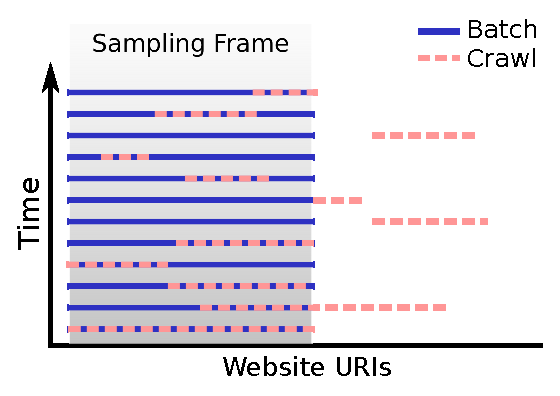
\includegraphics[width=0.8\textwidth]{longitudinal/lwac-samples}
    \caption{URI coverage for batch and crawl}
    \label{fig:longitudinal:lwac:samples}
\end{figure}

This approach allows for reliable re-visits to each member of the sample, and thus the construction of vertically comparable data points, whilst making short-term effects visible by revisiting each link.  Such a sample design should repeat each individual sample as quickly as possible, so as to minimise the time differences between documents within.

\til{Continue writing up `LWAC' slides from here}


\section{Applications}
Our strategy allows us to investigate how language may change in relation to technical and social events in a way that mimics the experience of the end user, and offers a useful perspective on many epistemic problems of WaC methods, to determine:

\begin{itemize}
    \item The portions of web pages that typically change as main content regions;
        \vspace{-6pt}
    \item The impact of social feedback and user generated content on page content;
        \vspace{-6pt}
    \item How censorship, redaction and revision affect website contents;
        \vspace{-6pt}
    \item Website resource persistence and its relation to linguistic content (link rot/document attrition);
        \vspace{-6pt}
    \item How institutions' publishing policies affect reporting of current events.
\end{itemize}

In order to maximise its coverage of these topics, LWAC~is designed to construct longitudinal samples from arbitrary URI lists, using commodity hardware, in a way that mimics the user's experience of a website.  


% The tool is designed to construct longitudinal samples from URI lists, using only commodity hardware.  It is designed with `full storage' in mind, that is, recording everything about each HTTP session in such a way that it may later be exported and accessed in a parsimonious manner.







\subsection{Design \& Implementation}


\begin{figure}[Ht]
    \centering
    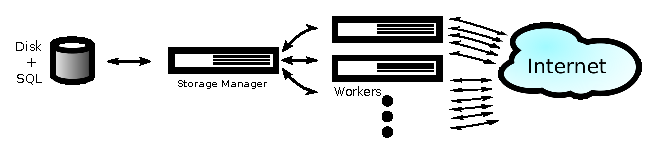
\includegraphics[width=0.8\textwidth]{longitudinal/lwac-arch}
    \caption{System Architecture}
    \label{fig:longitudinal:lwac:arch}
\end{figure}

In order to form a useful longitudinal sample, each data point should be as time-invariate as possible.  As such, a highly parallel, distributed architecture was selected (Figure~\ref{fig:longitudinal:lwac:arch}).  This yields technical benefits in terms of throughput (especially where the internet connection is a bottleneck), flexibility, and the ability to differentiate between websites that are blocked for a given area of the internet and those that are offline proper.

Data storage in the system is split between metadata, stored in an SQL database, and website sample data itself, which is stored as raw HTTP response data in a versioned structure on disk.  The storage format is optimised for large samples, and is nested in order to avoid common filesystem limits.  LWAC~does not enumerate URIs in memory, meaning there is no hard limit on corpus size.

The download process is managed by a central server, which co-ordinates storage and metadata access and provides full atomicity.  This server distributes batch jobs, according to policies governing reliability and throughput, to worker clients, which compete for the opportunity to download web pages.

Workers are able to imitate the behaviour of end users' browsers as much as possible, so as to avoid search engine optimisation and user-agent detection tactics (for example, they may retain cookies and present typical request headers).

After downloads have occurred, data may be retrieved for analysis in a variety of formats using the included export tool.






\subsection{Performance}


\subsection{Summary}







\section{Summary}
\label{sec:longitudinal:summary}
Mention which of these are to be selected and why, link to later chapters.



\chapter{Proportionality: A Case Study}
\label{sec:personal}
\section{Introduction}
The degree to which a general purpose corpus represents ``real'' language use is often debated at length, and is the key issue affecting design of corpora.  A wide variety of methods have been used to estimate language proportions and usage for a whole population, however, these are mediated by (and often centre around), expert opinion.

Reasons for this approach are both theoretical and practical---sampling individuals in the act of using language is very difficult (something other social sciences also struggle with), and the persistent nature of texts means that they conceptually stand alone, especially where the corpus designers intend to include older works.

Nonetheless, there is a missing empirical link between the expert-guided designs of language proportions and the ground truth of an individual's language use.  This is lamented by many who wish to study language acquisition (or more detailed explanatory theories regarding language use over time \td{cite Hoey, quote too}.

This chapter describes a case study whereby a census of text types was attempted for a single individual.  This sample design yields very little inferential power regarding the whole population, but serves to illustrate the disparity between the proportions a general purpose corpus may have, and the language used by an example individual.  The extent to which this example individual may be a useful guide for corpus building is not addressed directly, but this is an area that could be expanded using demographic auxiliary data.















% ============================================================================
\section{Sample Design}
As we have seen in chapters~\ref{}\td{ref}, conventional corpus building efforts centre around linguistic variables, and rely largely on expert opinion to balance their socioeconomic variables.  This approach was initially selected in order to avoid certain practical problems (many of them caused by technological limitations), though it has also caused others, most notably the difficulty in retrieving metadata about texts post-hoc.

Often, the only way to ensure demographic balance is to rely on sources of auxiliary data such as bestseller lists and library loan records that map textual variables to socioeconomic ones.  This process of using `proxy' variables is particularly opaque, and often limits the metadata available.

The intent of this chapter is to sample in an ad-hoc manner, that is, to record details of a text or single use of language in context, as it is used.  This approach is far closer to that used in special purpose corpora, especially where the restricted domain allows use of automated recording tools or sampling from an existing rich database (such as from an online forum).

The case study itself takes the form of a census of language use, for a given period, for a given person.  This offers empirical validity for linguistic proportions, but is a single data point from the population of language users and cannot be formally generalised.

Of particular interest are variables that are particularly challenging to sample:

\begin{itemize}
    \item The age of a text when ``used''
    \item Other temporal information, such as the times and days when texts are read, and inter-day variance etc.
    \item The social context of text use
    \item Attention paid to a text, and which portions were read
    \item Proportions of text types used, especially representation of types that may be missing from other corpora such as greetings, billboards, product labels.
\end{itemize}

The ad-hoc sampling approach, applied to \textsl{all} texts used, also allows inspection of the proportions of language types used---something that is estimated for general purpose corpora.  Though the scope of this case study is necessarily limited, a ``language use census'' for many people would be a robust empirical method for validating claims of representativeness in GP corpora.


A further advantage of this method is that the population may be rigorously defined, as data on the participants is available to whatever standard deemed necessary.  This is notably at odds with the use of existing lists or repositories, which have been constructed with differing purposes and levels of documentation.






\subsection{Difficulties and Disadvantages}
Sampling language use ad-hoc involves changes in sampling strategy that are practically challenging.  Taking this study as an example, one would have to take data from enough people to cover the population required, and each would have to undertake a fairly in-depth procedure.

Difficulties encountered when trying to sample large populations are well documented in the social sciences, and many techniques exist to mitigate common biases (\td{such as}), however, these are largely beyond the scope of this chapter.  It is notable that one solution in sociology has been to share data (in a style similar to corpus linguistics) in order to minimise the costs involved in implementing a high quality survey.

The increased ``person-focused''ness of a primarily social design also raises a number of ethical issues, as it is increasingly possible to derive information not just about a general group's language preferences, but about an individual's (or a comparison between groups).  This is merely the inverse of its value, but it is nonetheless worth considering as many study designs in linguistics need not work with such sensitive data.  This issue is addressed after the discussion of methods and findings\td{Ensure that it is.}.

Further, sampling text as it is used raises methodological challenges---how can we be sure that the language observed is still naturally occurring and valid?  All sampling is going to compromise on this, and the extent to which one values detail over interruption will vary by study design.  The aims of this study are, in part, to identify major challenges in this area, for example, which text types are most difficult to sample or require most time to record.














% ============================================================================
\section{Technology}
As mentioned, a number of the limitations to this kind of sampling may be addressed through the application of new and emerging technologies.  This takes two main forms:

\begin{itemize}
    \item Many more documents are now poduced and consumed in digital form.  This means they are accessible for automatic copying and processing by sampling software, often without any intervention necessary by the user.
    \item The abundance and ubiquity of portable technology such as smartphones lowers the difficulty of many existing sampling methods such as audio recording or photography.
\end{itemize}


The former of these is well represented by the WaC movement in corpus linguistics, and many corpora include sections which have been sampled by distributing portable technology\til{So, er, this is where the lit review seems out of place 'cause it's in chapter 2}.  Of particular interest, however, is the value that we may extract by exploiting both to form a coherent narrative.

One community that has been using these techniques extensively is that associated with life-logging.  Life-loggers do stuff---see lit review.










\subsection{Life Logging}
Just as the availability of portable recording technology made acquisition of spoken corpora relatively easy to control, so have the limitations on digitisation and format conversion limited the selection of written text to those already-indexed properties.  As modern computing devices have miniturised and become ubiquitous, they have developed a number of capacities that may be used to afford the same ``instantly recordable'' status to non-spoken language use.


A number of these technologies are as a direct result of the life-logging community's interest in multimedia records.  Life logging is an activity that emerged slowly out of the principles of webcam shows and reality TV.  It involves recording (and usually broadcasting) continuous information about one's life as it occurs.

Though most popular efforts started as a means for providing entertainment, and thus focused on multimedia broadcasting on the web, the techniques required soon diversified and gained the interest of the information retrieval and processing communities.  Many projects have been started with an aim to catalogue and operationalise the huge stream of data each person creates, largely with a focus on aiding that person in their daily life, or aiding large organisations (such as defence forces) in management of resources and people.

\til{citations and a proper lit review, but they are maybe better off elsewhere}

Because of the continuous nature of life-logging, many efforts have been made to use methods that are easy to maintain, self-contained, and covert.  % CITE
Due to this, as well as the original intent of the life-logging process, much of the effort surrounding life-logging focuses on multi-media sources, and how they may be best combined to form a coherent idea of context.  

Typical sources of data considered include:

\begin{itemizeTitle}
    \item[Video recording] Many life-loggers wear systems that are able to continuously record video in the direction they look, and upload this using mobile networking systems.
    \item[Audio recording] Due to its lower obtrusivity, many efforts surround the analysis of audio logs, and include systems to detect voices and identify events such as making appointments.
    \item[Document storage] With the increase in use of digital-origin documents, some of the more holistic life-logging systems record documents as they are read, with a focus being to integrate this data into the larger picture.  Others scan in their post for later retrieval.
\end{itemizeTitle}

Many of the requirements of a life-logging platform (covert operation, comprehensive data management, context identification) overlap notably with the methods used in covert sociological research and, of particular note for our purposes, those constructing spoken language corpora.

Notably, one of the methods used to create the spoken portion of the BNC was covert recording, where a number of people were provided with tape recorders...
\til{ Quote from BNC documentation }

As illustrated by the BNC's demographic balancing of that portion of their corpus, this ability to directly record data from the field satisfies the disadvantages of text-index-oriented methods of document selection, allowing us access to all of the contextual data at the time of text consumption/production 
\til{perhaps because the time of production and consumption don't differ much for spoken stuff...}

The cost of this is, as felt by all sociological studies, a need to find a sufficiently large and heterogenous sample of people who may record data about their language use (and for long enough for it to be useful to researchers).  This is arguably more difficult in practice than text-index-based methods, and should only be considered at a large scale where the difference is likely to be crucial to a study, nonetheless, large samples exist in sociology as testament to the value such designs may yield [and the illustration that no alternative method exists for many sociological issues].

The benefit of having a clearly-defined population about which to generalise linguistic findings is applicable to any size sample, however, making techniques of logging particularly applicable to special-purpose corpora, especially where those corpora are best demarcked along social lines.  Indeed, at one extreme of this scale exists the concept of a personal corpus; something that may yield insights or models about a single person's current language usage.  Such a resource may one day be particularly valuable in defining how one uses text-based interactive systems (such as the web), reads content (such as news articles) or even how one would learn.

Such designs exhibit a tradeoff: a decrease in socioeconomic breadth in exchange for an increase in linguistic breadth.  It is my intent to illustrate the value in this approach, and to investigate methods by which it is possible to construct corpora without undue difficulty through the use of life-logging methods.
% This needs mega elucidation, methinks



\til{ Intro to life logging, a good lit review needs to be done.  Perhaps it belongs in the lit review section rather than here though.}

















% ============================================================================
\section{Approach \& RQs}
The case study described here is an attempt to assess the extent to which techniques from life-logging may assist corpus builders in creasing a demographically-oriented corpus.

It follows an iterative design surrounding these aims, with each iteration refining a number of key design areas:

\begin{itemize}
    \item The variables that may practically be recorded about a text (and that must be before they are lost);
    \item Methods that may be used to sample text unobtrusively, especially how new technologies may be used to assist;
    \item Methods and tools for operationalising logs after sampling is complete, and how these may assist the process of data gathering itself.
\end{itemize}
\til{I'm sure I'm missing stuff here.  Check notes and presentations}

Ultimately, the differences in sample design contribute to a larger picture that could yield much future work.  The direct research questions addressed here are:

\begin{itemize}
    \item What methods may be used for gathering data in a short-term language census?
    \item How may the collected data be operationalised?
    \item What proportions of language are used by the subject; do these support common claims from general purpose corpora?
    \item How may these methods be used in future to aid those building corpora?
\end{itemize}







\subsection{Sampling Policy}
\label{sec:personal:samplingpolicy}
\td{from notes}
The aim of a personal corpus is to emulate, as closely as possible, a census of observed language.

Use of language, in this context, is defined as any conveyance of information, spoken or written, in any quantity. There are no bounds to the context in which it is used, nor the language itself, as the purpose of the study is to evaluate these very things.

Each of these transactions is recorded as a single line in the data set, and will be annotated with the variables recorded.  One of the major issues encountered in preliminary tests was annotation for attention and proportions read.  These will be recorded along with textual properties to ease operationalisation.

Attempts were also made to record sufficient data to retrieve the full text of each transaction.  This worked better for some data sources, and much of the case study thus concerns itself with (sometimes estimated) word counts.  Word counts were chosen as a measure of size due to their use in other corpora, and their applicability to many different media.


A number of practical challenges were identified before sampling, and these were backed up by experience:
\begin{itemizeTitle}
    \item[Review and Production] Both should be recorded as fully as possible. Where a text is re-read, or developed and continually re-read, this should be noted as an ongoing process (and accordingly oversampled).
    \item[Short Utterances] Very short interactions, such as passing greetings, should not be under-recorded. Their inclusion is likely to be one major difference from conventional corpora.
    \item[Oft-reread Texts] such as labels, signs and the like. It’s debatable whether or not one actually reads or merely remembers/recognises these. Perhaps psychological literature (Gestalt, etc.) can shed some light on this?
% See Wang, Zhe, and Gemmell, Jim, Clean Living: Eliminating Near-Duplicates in Lifetime Personal Storage, Microsoft Research Technical Report MSR-TR-2006-30, March 2006.
\end{itemizeTitle}










% ============================================================================
\section{Method}
As mentioned in~\ref{sec:personal:samplingpolicy}, the primary objective of the sampling is to record all ``linguistic events'' for a given period, for a given subject.

The subject chosen was myself---this was done for a number of reasons:

Firstly, legal and ethical issues surrounding recording and review of the data were mitigated by having the analysis performed by a member of the original conversations, etc.

Secondly, iterative review of methods involved was possible with internal, `white box' examination of how data were collected, and what edge cases and procedural difficulties arose.

Thirdly, the demographic status and other person-related variables are well known and need no formal elicitation, minimising time spent on construction of questionnaires et al.


\subsection{Data Sources}
Before the first iteration of the sampling/review process, all of the possible language data sources used in everyday life of the subject were informally identified.  It soon became clear that these data sources exhibited properties that would make sampling easier, or less intrusive.  They were classified by the methods required to capture their text:

\begin{itemizeTitle}
    \item[Persistent] Resources that exist in a format that is easily retrieved and immutable.  This covers many physical items such as books, and some broadcast media as well as notes made in a notebook.  Only identifying information must be stored during sampling itself, in some cases merely an ISBN or similar index code.
    \item[Ephemeral] Language data that cannot be accessed after-the-fact in any way, or may differ by time or context.  This most obviously contains speech, but also many websites, things such as billboards that cannot be readily re-accessed, or todo lists that get destroyed.
    \item[Digital Origin] Documents that are read, or written, on electronic devices.  These may fall into either of the above categories, yet they may usually be copied with no overhead so it is often simpler to store them at the time of use.  Many document types are now digital, as well as the obvious sources such as email or online chat.
\end{itemizeTitle}

This classification was useful in order to minimise the intrusiveness of a collection method, whilst maximising the detail recorded for a given source (ideally to the point of storing verbatim text).  In practice, methods were easy to develop for automated recording of digital documents, and many techniques exist for sampling non-digital persistent and ephemeral sources with scientific levels of accuracy already.

The sources identified in the initial case study were as follows:

\td{Merge these two lists with a separator or something?}
\begin{itemize}
    \item Speech
    \item Printed documents (i.e.\ letters, brochures)
    \item Digital documents (same, but unprinted)
    \item Terminal logs
    \item IRC logs
    \item Email
    \item Websites
    \item Unusually formatted printed material (posters, labels, advertising on vehicles, billboards, etc.)
\end{itemize}

The inadequacies of introspective methods to identify these soon became apparent during preliminary tests, as the process of recording increased awareness of language use, raising a series of edge cases.  These were collected and resulted in a final selection of sources displayed below.  As well as expending the set of sources to be gathered, methods of collection were chosen with flexibility in mind in order to cope with unenvisaged sources of data\footnote{This flexibility has the unwelcome effect of slowing down analysis later on, and may be undesirable in some cases}.


\begin{figure}[p]
\centering
\includegraphics[width=0.4\textwidth]{datasources}
\caption{Data sources and their appropriate capture methods}
\label{fig:personal:datasources}
\end{figure}



\begin{itemize}
    \item Speech
    \item Printed documents (i.e.\ letters, brochures)
    \item Digital documents (same, but unprinted)
    \item Terminal logs
    \item IRC logs
    \item Email
    \item Websites
    \item Unusually formatted printed material (posters, labels, advertising on vehicles, billboards, etc.)
    %---
    \item Written (but non-OCRable) material
    \item Key strokes
    \item SMS records
    \item Phone conversations (separated from speech as they yield differing metadata)
    \item Music tracks
    \item Files accessed
\end{itemize}

This list is necessarily furnished according to the life of the subject in question---from this study I am unable to assert that it is generalisable to others, though the process of doing so would involve relatively little intrusive sampling\td{link to further work}.

Each of these sources is ``covered'' by one or more sampling tools.  These tools progressed most during the iterative process, and each was subject to a number of procedural subtleties that were refined throughout the study.


\til{Diagram from notebook, figure~\ref{fig:personal:datasources}}










\subsection{Recording Methods}
Recording methods were chosen for a variety of reasons.  First and foremost they must, in sum, cover the sources mentioned above.  Secondly, they were selected in order to be unobtrusive both for the experimenter and those around him.  Thirdly, they were selected to be flexible enough to cover unforseen contexts and data sources.

The methods used can be separated further into two groups: many methods are capable of recording multiple sources, and serve to form a narrative that describes the metadata of a linguistic event, pointing at another source for the data itself.  These methods were chosen to allow for post-hoc ``memory jogging'' and narrative creation, something that was added to the experimental procedure after the first iteration indicated how difficult to operationalise much of the data would be.

The second set of methods are focused on a single data source, typically requiring little to no manual intervention to record it.  Their records are either indexed by time, or by the more flexible methods mentioned above.


\subsubsection{Indexing and Overview}
\paragraph{Journals and Note-taking}

\begin{figure}[p]
\centering
\includegraphics[width=0.8\textwidth]{notebook}
\caption{The `on-line' notebook}
\label{fig:personal:online_notebook}
\end{figure}

Two journals were maintained throughout the sample.  The former of these was an A6 notebook maintained `on-line'\td{rename to hot/warm/cold, front/mid/backline or something similar} as events occurred (pictured in figure~\ref{fig:personal:online_notebook}).  This was used to store durations of conversations, titles of persistent sources, etc.

The second was an off-line journal, maintained at the end of each day in a narrative style.  This blog-like record was intended to reflect in depth on the proportions of text used in each source, and how attentively each linguistic event was engaged in.  The writing of the journal itself was not logged by any other methods.  It was also possible to attach daily records to this journal, and the process of writing it inserted an opportunity to reflect on the mnemonic codes used during the day.  This process is described in context in section~\ref{sec:personal:recording}.

The on-line notebook proved to be the primary indexing method for all other sources of data, and its maintenance was the primary overhead of the study.  Each entry in the notebook was eventually reduced to a compressed form that roughly followed one-line-per-event, storing the time each event occurred, any identifying information deemed necessary for later memory of it, and a duration or other index of word counts.

\til{Insert a picture of one of the scanned days, pointing out the format}

Problems of simultaneous events and split attention were solved in the notes by having a start/stop event for ongoing events, and by using the off-line journal to reflect upon each event.


\paragraph{Audio Recording}
Following work on machine listening, the original intent of audio recording was to capture the occurrence and duration of conversations, as well as any smaller interactions that would otherwise be difficult to capture (such as greetings, thanks when opening doors, etc.)


\begin{figure}[p]
\centering
\includegraphics[width=0.8\textwidth]{dictaphone}
\caption{The audio recorder used}
\label{fig:personal:audiorecorder}
\end{figure}



Capturing was performed with an Olympus 713PC\td{check this, is it PC713?} dictaphone, recording to a suitably sized external card that yielded many days' continuous recording.  Provision was made to download recordings each night and store them with the off-line journal, however, in practice they remained on the recorder until the end of the study.


\begin{figure}[p]
\centering
\includegraphics[width=0.8\textwidth]{clicker}
\caption{The second audio index marker}
\label{fig:personal:clicker}
\end{figure}


Aligning the recorder's output to the events mentioned in the notebook was a tricky process---Though the recorder itself supports index marks, there is a limit of 99, which was deemed riskily low.  Two devices were built to insert absolute silence onto the recording (something that is rare in real life and easy to programmatically detect), the later of which is pictured in figure~\ref{fig:personal:clicker}.  These clickers were to be pressed at the beginning of each conversation, so that voice activity detection could be performed to estimate the word count of each conversation (or, in an ideal world, extract verbatim text).

In practice, the process of tapping the button proved intrusive and, from the perspective of one talking to the subject, suspicious.

The mechanism used for the final iteration of the study was far simpler---the recorder's start time was written in the on-line notebook, and entries therein were keyed by computing the offset between the two times.  Though this incurs a minor overhead in coding the data, it also allows for spontaneous conversations without much overhead, something that is particularly important to the study of text type proportions.



\paragraph{Photographs}
The primary method of capturing ephemeral, irregularly formatted, non-digital texts was photography using a cameraphone.  This method was chosen largely because the ubiquity of smartphones in British society has led to a situation where photographing fairly mundane items is widely unquestioned.

The smartphone used, a Motorola Milestone, also stores time and location data in its photographs using EXIF tags (as well as storing photographs sorted by day).  This metadata meant that there was often no need to file an entry in the on-line notebook, and the cameraphone could simply be used in a very unobtrusive ad-hoc manner.

In earlier iterations of the study, it became apparent that the loud shutter noise made by the Android operating system when taking photographs was problematic.  Though photography of signs, packets and such remained unchallenged, the attention of people nearby was drawn to the weirdo with the cameraphone all too readily.  This was solved partially by (with great difficulty) disabling the noise, though it was still apparent from posture when a photograph was being taken.

There are notably a number of products available that continually take photographs for the purposes of life logging.  These were considered for the study, but their aims are generally to capture each event, rather than specific aspects of selected scenarios.  The ability to consciously specify that the subject was more attentive in some situations (and take pictures accordingly) was judged to outweigh the value of having a continuous record (something much more capably performed by the journals).




\subsubsection{Targeted Methods}
\paragraph{Phone Calls \& SMS Messages}
Both of these are automatically logged by the Android operating system used by the subject, and each was also indexed in the on-line notebook.  The data was extracted using a free application that exported to XML.


\paragraph{IRC}
IRC was logged by construction of a bot.  This bot accompanies the subject into chatrooms and logs all messages observed, applying a rough human interest model to ignore data seen when the user is set to away.


\paragraph{Web}
The SQUID webproxy was configured to log all traffic, and a number of logins were provided---one for each of the subject's internet-enabled devices.

The logs from SQUID store all requests, including advertising/tracking calls, downloading of things never read by the user (i.e. CSS and Javascript) and AJAX calls to partially reload pages.  As such, a large amount of processing was necessary to extract URLs from these logs, and to parse the resultant data into a usable format.

\paragraph{Keylogging/Terminal recording}
Terminals and keyboard input were logged using a custom application that wrapped a terminal, recording the time each character was sent or received to the shell.

Each terminal created started recording to a new log file, storing the time at which it was started and a series of offsets from this time.

\paragraph{Last.fm}
In earlier iterations it was apparent that lyrics in music were being missed as a source of text---all devices capable of playing music were configured to `scrobble' to the last.fm music service during the sampling period.

Though last.fm do not make their data freely available for access, third party tools exist to scrape their website and download detailed logs of tracks listened to.

\paragraph{Files}
Files were identified in a number of ways.

Some, particularly those on which the subject worked and contributed data, were written down in the journals.  This is a precise method of separating what has been read, but might require a large overhead.

Since the subject works entirely on projects and files that reside in a RCS repository, the logs from each commit were used to generate a diff, and this was accessed after the sampling period to identify contributions made.

Another policy that may be used is identification of files by unix mtime (modification) or ctime (creation), however, this is fraught with inaccuracy, as files are liable to be modified on disk many times whilst being edited, and sampling the differences is likely to happen at haphazard times.  Further, this technique would capture many log files and others that have been edited by processes where the subject was not involved linguistically.  By contrast, commits to an RCS are scheduled around logical additions, and are manually pushed so that only deliberately edited files are stored.

Files uploaded whilst on other systems may be uploaded directly to the off-line journal (which, ironically, is online), or stored on a flash drive that was carried specifically for the purpose.  In practice this did not occur during the recording period, though experience suggests these contingencies would be necessary if a longer sample were taken.

\paragraph{Email}
Emails are, again, stored automatically with sufficient metadata as to make them self-documenting.  However, rather than presume all were read in a given day, each was tagged after being read with a label corresponding to the day.

At the end of the sampling period, these tags were collected and downloaded in mbox format, whence they were processed by the operationalisation script.









\subsection{Recording Procedure}
\label{sec:personal:recording}
The study is based around a period of continuous sampling using the methods discussed above.  For two weeks (in some cases longer), data was captured for each source.  This process was structured around a daily routine:

Upon waking, and before any language was used, the recorder was turned on and a note of the time at which this occurred was made in the on-line notebook.  Recording was then continued until the end of the day without interruption.

The on-line notebook, cameraphone, and flash drive, were carried at all times.  Since each of these could be backed up (the cameraphone even did this backup automatically), the most data at risk was a single day.

Notebook entries were made as soon as was possible without interrupting the linguistic event being recorded.

At the end of the day (immediately prior to sleep), a journal entry was written in the off-line journal, and SQUID logs were uploaded for the day.  This journal entry forms a narrative, estimating the time taken and attention paid to items in the on-line journal for that day, as well as detailing anything that may be written in shorthand-mnemonic form.










\subsection{Operationalisation, Processing and Analysis}
Normalising and operationalising such heterogenous data without significant overhead proved to be a significant problem that was only partially solved, and the data set presented here required significant manual intervention that was possible in part due to the fact that the analyst was the subject.

This advantage, clearly, cannot be relied upon in other studies, and this part of the method demands most further study in order to define typical parameters for many processes that are dependent on human properties.

Two main processes were followed in data processing.  The former of these was aggregation and normalisation---each data source was collected and transformed into a one-event-per-line CSV containing a standard set of fields (the selection of fields used was modelled on Lee's BNC index\td{CITE} in order to facilitate comparison).

After this normalisation process was complete, data were manually annotated to complete any fields that were not stored in the original metadata.  This was largely an objective, uncreative task that simply demanded human reasoning capacity, but it is inevitable that some bias will creep in at this stage.

The second stage of processing involved coding text types and roles.  This task is altogether more flexible and subject to design errors and bias than many of the normalisation stages, and was thus attempted in a manner that was designed beforehand.  Since the aim of this study is, in part, to identify text types not seen in other corpora, following an existing taxonomy would necessarily limit the coding of any newly discovered.  True free coding, however, is likely to draw distinctions between text types that are not made in existing taxonomies, rendering them incomparable.

The process followed was a hybrid approach---data were freely coded by inspection of the texts, but this was done with deliberate prior knowledge of Lee's classification scheme.  The intent was to categorise texts according to Lee's scheme only in so far as they were deemed suitable by the analyst (who is also, lest we forget, the subject).

Though this approach was suitable for the aims of this particular study, it is difficult to advocate for any others using the sampling techniques described, and its use here should not be taken as such.

%---
\subsubsection{Human Interest Models}
Beyond coding, by far the largest single influence on the data recorded was the human interest model applied.  This was created in order to take into account two factors that had become particularly apparent (and notably do not apply in the same manner to conventional corpus designs, where many eyes may cover a whole document in sum):

\begin{itemize}
    \item Often, only small (usually predictable) portions of a text are used.  For example, I have started to read more books than I have finished reading.  Generalised, this means that even Brown-designed corpora should favour the start of their texts slightly when selecting excerpts.  Some media were more surceptible to this than others, and the automated normalisation tools were built with facilities to take this into account.
    \item Texts, especially broadcast media and speech, were often used whilst also accomplishing a non-textual task (or sometimes both at once, such as talking with the radio on in the background).
\end{itemize}

Both of these were noted in journals, and added to the processing toolchain---each data source's normalisation script contained a model to extract the portions of text that were read, and each row of the normalised data format contained an ``attention index'', ranging from 0--1, that served as a coefficient of the word count.

Though crude, this measure was able to produce approximations for word counts that were inline with the expectations of the subject.  (It is recognised that this may not hold much scientific value to others wishing to replicate the study, and in general it is necessary to investigate the inter-person variability of these properties in order to create more generalised processing tools.)


% TODO: perhaps a run-down of each annotation program?
\paragraph{Web logs}
The human interest model for web logging was built by inspection of the web logs and cross-referencing with information about the hosts identified.  The normalisation script is concerned primarily with removing material that was downloaded without ever having been viewed, for example, non-text MIME types and advertising, and contains a multi-stage strategy for excluding content:

\begin{enumerate}
    \item Filter only successful requests
    \item Filter only those requests that are of textual mime types (\texttt{text/*})
    \item Apply a blacklist of advertising websites and file extensions (manually constructed)
    \item Discard links where the page was reloaded and the URL is the same as the previous entry in the list (this pattern is often caused by initially connecting to the proxy, for example)
    \item Non-visible text items were discarded (non-body elements if the file is HTML), and markup was removed
\end{enumerate}

Beyond this initial normalisation, a speadsheet's \texttt{LOOKUP} function was used to manually assign attention coefficients to the domains, based upon entries in the journals and interesting portions of web pages that follow regular structures.

Days were classified as changing at 4am, since there were no points in the data set where the subject was still using the web at this time.



\paragraph{IRC Logs}
IRC logs were already stored using a limited attention model, which was based on the principle that, in IRC, conversations are started, live for a short time, then die off as people in the channel return to work.  The bot performing logging would start logging (and continue to log) for as long as the subject was talking, stopping 10 minutes after the final utterance.

In order to capture a human notion of day, that is, one demarked by sleep rather than midnight, the start time of each conversation was used to determine the day its data fell into.



\paragraph{Terminal [Console] logs}
Terminal data was logged with timestamps on each individual character, and the model was thus responsible for inferring when a command had output, and suggesting which portions of text were still on screen.

This was done with a `timeout' and a `scrollback'---the former describing a delay that had to be present for the text to have been read (rather than simply scrolling offscreen), and the latter describing the average size of a terminal (and thus the number of rows of text that remain displayed).

These parameters were tuned to match the specific data sampled over the period---for example, the time recorded included terminal use displaying logs from software that was being developed, and these would produce thousands of lines of output before a pause.



% \paragraph{}





\section{Results}

\begin{figure}[p]
\centering
\includegraphics[width=0.8\textwidth]{dataoverview}
\caption{The availability of data from various sources}
\label{fig:personal:dataoverview}
\end{figure}


These results describe data collected during the third iteration of sampling, which lasted roughly two weeks during April 2013.  Table~\ref{figure:personal:dataoverview}\td{make into a table} describes the availability of data per-day.

The period marked from Friday the 5th to Friday the 19th (inclusive) forms the sampling period described herein (with exceptions to this noted where made).  This was the period for which the on-line notebook was maintained along with other intrusive data collection techniques, though notably some methods continued due to their ease-of-use.

Though audio data is missing for Friday 19th, this was not used due to the difficulty in processing such data ethically and within a reasonable time frame.  Word counts for spoken transactions were instead based on an estimated words-per-minute.  /%XXX: revisit this and do manual transcription some day before the viva?

This fifteen-day recording period covers 8,619 linguistic events, encompassing an estimated 980,000 words.  



\subsection{Variables}
Variables recorded on each linguistic event are based heavily on Lee's BNC index, augmented to take into account the attention index and word count estimates.

\til{table of variables}



\subsection{Activities}
During the sampling period, all work surrounding the personal corpus case study was stopped, in favour of other, ongoing, projects.  Other than this intervention, work continued as normal, which for this period involved significant amounts of development on the LWAC downloader tool.

% TODO: more about genera life in that period





\subsection{Frequencies and Summaries}
\til{See presentation for a few breakdowns.

Also do more word count comparisons against things such as the BNC.  Possibly also pick out some demographics and compare only to people like me.
}







\subsection{Specific RQs...}

\til{Notes suggest uses: 

* Stratified Comparison
* Synchronic Comparison
* Vocabulary estimation
* 'learning rate' estimation for some features (learner corpus stuff)
}


\til{ Technical problems,
    coding problems,
    what did I read/not read?,
    What proportions were missing/over/under represented,
}


\subsection{Discussion}

\til{qualitative findings...}
\subsection{}



\subsection{Validity}
The design of this experiment is subject to a number of challenges to validity, and is presented in an explanatory context.

* The proportions used are estimated and based on my subjective opinion
* When something is formally `read' is based on my subjective opinion
* Generalisability is low to others
* Any inference drawn from comparison to other corpora can be done rationally only, as quantiative data does not exist on inter-person variability



\subsection{Ethics}
The increased resolution of data pertaining to a single individual renders the methods discussed here ethically sensitive.  This sensitivity is increased further if continuous recording of audio or video are used, though, as mentioned above, this data was not integrated into my analysis.

There are a number of arguments justifying covert research in the social sciences, and ...




Further, future developments in the methods described may use questionnaires or other less-invasive methods as sources of auxiliary data.  These would be targeted to a particular study design and need not cover the full set of language uses, mitigating any ethical concerns by limiting the descriptive power of the raw data itself.

A number of technical measures are also possible that may assist this issue---some of these have been developed by \td{who} working on the Machine Listening project, who irreversably scramble their audio recordings in such a way that VAD algorithms may still run.  A further option is streaming of data to a remote server, which can process, summarise, and discard data on-the-fly to prevent any possible information security breaches.








% ============================================================================
\section{Future Work}

In the long term, it is hoped that a greater understanding of the above may contribute to:

\begin{itemize}
    \item Methods for augmenting and rebalancing corpora using a questionnaire or other surrogate auxiliary data
    \item A greater understanding of variance in terms of the populations being studied
    \item 
\end{itemize}

From a sample of just one person, it is possible to use auxiliary data from existing sources to operationalise and reason about inter-person variability.  This may be done by cross-referencing a subject's demographic variables with those from an existing corpus, placing them in context and allowing comparison of his linguistic data to other groups (or to those within a given similarity).

This technique can also be used to impute data from partially-sampled sources, creating a personal corpus by re-weighting existing samples.

Unfortunately many existing corpora are unsuitable for this process due to the limited availability of metadata (something that is also an issue for those constructing ``informal'' subsets).






% ============================================================================
\section{Summary}













\section{--- --- ---}
% 
% \section{Intro/review stuff}
% 
% There is some discussion about the value of proportionality in corpus building.  The web makes this discussion particularly interesting, as the availability of pages online is different to those in general life (for any web user, a sizable subset).
% 
% Using the methods above, it should be possible to control for the proportions of language used in daily life, to construct a corpus from these that is both web-sourced (and hence easy to sample) and yet balanced to a given population.  This is, in effect, the goal of many special purpose corpora sampled online.
% 
\section{Methods for Proportional Selection Online}
Many web-as-corpus tools make at best modest efforts to constrain their output.  There are a number of good reasons for this:

\paragraph{Metadata Availability}
Many of the variables available for balancing data online are of limited applicabilty to many corpus objectives: consider, for example, the data attached to many web pages, which is typically limited to the HTTP headers, location, and immediate context.  Many users will combine knowledge about the world and intuitions regarding content to judge the genre, author, and many other salient properties---something that is beyond the scope of many WaC processing toolchains.

This has been adjusted for using various methods, such as:

\begin{itemize}
    \item Selection of only certain top-level-domains (i.e. those for a given country)
    \item Use of HTTP headers to identify language or location of servers (limited due to poor coverage of internationalisation technologies)
    \item Use of metadata and non-content HTML body data (applicable only where services make a layout/content distinction)
    \item Heuristics (such as keyword counting in various languages; suitable only for simple inferences)
\end{itemize}


\paragraph{Internal Variables}
The problem of metadata availability is compounded further by the need to select documents without systematic linguistic bias (especially where general-purpose corpora are concerned).  Many available properties of web documents are essentially internal variables, and should not be used for sampling.

One method for controlling for this relies on seed terms, where a search engine will be used to find pages containing various collocations from a corpus.  This method is essentially a complex heuristic, and is reliant either on the principle that search engines will duplicate external variables by summary of the content they select, or that the content will be summarised from the original document and selected without bias by the search engine.  In practice this method proves fast, easy, and able to control (at least to some extent) for more complex characterisation than the coarse definitions covered by page metadata.  This method is boosted further by the existence of boilerlate/non-content text in pages, which may prove cause for selection without itself being content for the corpus.

\paragraph{Format Heterogeniety}
The format of web data is particularly heterogeneous, and this poses significant problems with respect to selection of pages based on their layout or appearance.  Without further (arbitrary) restriction by corpus compilers, the only common interface data online is designed for is the human eye (and some content even violates this assumption\footnote{Such as large dumps of tables, or things like JSON and XML serialisation formats.  Largely it is assumed that these will be excluded from the corpus by design anyway}).  

This means that any use of boilerplate and data surrounding the content itself is severely limited by our capacity to codify and process such a distinction---something that is easy for a corpus with few sources, but difficult for larger ones sampling wider population of text.

\paragraph{Population Ambiguity}
As mentioned in [the special edition on web as corpus], web corpora may be seen, strictly, as only representative of web content.  The extent to which this applies in practice is a matter of debate.

Those who spider the web, such as WebCorp and other services, offer corpora that are perhaps most closely tied to its layout and content---they do not make any efforts to (re-)balance their corpora in terms of other proportions, and subsequently end up with a natural representation of web data.

Users of techniques such as those mentioned above are able to apply weighted selection policies to correct for this, however, the extent to which this is capable of correcting for the web's idiosynchrasies is debatable---issues of presentation (``click here") and context are at play for which there is no alternative source of data online, and this necessarily limits the power of any methods for mitigating differences between `real life' and web corpora. % TODO: rephrase and shorten
\til{More stuff, elucidate more especially on this point since it's pretty crucial to the narrative} 

% 
% \section{Establishing Proportions of Strata}
% The proportions of corpora have traditionally been established through a combination of experiment, debate, and reason.  This process has been well documented in the early corpora, \todo{ read up on some examples to include here}
% 
% 
% As with most aspects of corpus construction, practical limitations necessarily restrict the selection and variety of data sources available.  This has conventionally led to selection from large pre-indexed resources such as library catalogues, publisher's records, and bestseller lists.  We may see this stratification of variables as being primarily governed by the proportional consumption of text types, measuring the population's socioeconomically-influenced consumption of text by the text's popularity.
% 
% This method is contrary to many other samples in social science, which seek primarily to control for a given socioeconomically-defined population.  In the case of text corpora, the reasoning behind this is doubtless often pragmatic: it is far cheaper and simpler to rely on existing indexes, and brings us one step closer to gathering actual real-world book statistics.  This decision, then, may be seen as a generally wise and productive one for corpus linguistics, as it has freed the field from the need to fund and maintain even larger projects akin to the British Household Panel Survey or cohort studies.
% 
% Nonetheless, there are a number of disadvantages associated with this selection of variables.  One of the most pronounced scientifically is the definition of population: selecting primarily in terms of textual variables leads us to define our population in such a way, something that leads to an ambiguity in the boundaries of representation for the corpus, and the limits of generalisability for any resultant conclusions.  This effects is especially pronounced for special-purpose corpora, about which generalisations must be qualified with much greater specificity.
% 
% Other disadvantages with this method surround the power socioeconomic annotation gives to those using corpus resources.  Often, simpler annotations derived from text-oriented variables are insufficient to drill-down into a ``Who uses what'' question format, something that may be crucial in reducing within-class variance to the point where many techniques are useful.
% 
% Another property obscured by description in terms of texts is the differentiation between text production/performance and reception.  This distinction is well noted in corpus documentation (going back to Brown... % TODO: quote
% ), but, except in circumstances where the distinction is of particular interest, often compromised.  Designs for corpora including Brown and the BNC state that their aim is to sample a ``mix'' of the two, so as to represent language use for the population (this is one major reason they take into account the relative popularity of works when selecting texts).  The lack of detail in this method denies any detailed inquiry into the ratio of text production and consumption, and any analyses and insights that lead from this.  Simply put, selection of texts from text-centric central indexes obscures this distinction.
% 
% \til{It might be wise to expand this section to debate the difficulties in text selection proportionally.  Also mention Leech, review things like the Czech NC}
% 
% It's worth noting here that the approach taken for written resources often differs to that for spoken.  The transient nature of spoken language mandates capture during performance, meaning that little of it is indexed.  Many spoken corpora thus contain data that was gathered by the authors themselves, affording an opportunity to both describe and balance the socioeconomic variables first with little effort.
% 
% As such, many spoken corpora are primarily oriented around these variables (in addition to text-format ones), for example the BNC's section, LLC, etc.  \todo{find examples}








% 
% \til{ talk about this allowing us to go out into the field and re-examine language use with less interruption,
%     the ability to get empirical data on text proportinoality,
%     lack of a need for a central index,
%     better population definition
% }
% 




\section{Scope}
The methods presented here are intended as an inspection of the issues that surround construction of personalised corpora, and should be seen as a first step towards the principles of building a ``socially balanced'' set of important variables across which to sample.  






\til{What aspects are in common with typical fieldwork?

Why stop where I did?

How long to sample for? Why?

Data sources.
}









% ============================================================================
\section{Method}
In order to best derive methods of data recording that were practical and well-suited to the lifestyle of the subject, experimental design proceeded in an iterative fashion.  Ultimately there were two formal preliminary data gathering stages, and after each of these a summary was written to alter the procedure for the next.





\til{What I did, like...
Should I describe the first preliminary approach as an iterative things?
}

\subsection{Variable Selection}
Variables selected for recording in the preliminary study were selected to be in line with those most commonly included in general-purpose corpora.  The decision was made to limit the number of these variables to facilitate unobtrusive recording (and maximise the relevance to the many different media recorded).



\til{Which variables I have tried to record and why}


\subsection{Capture Methods}
\til{ \\paragraph{}-ised list of methods }



\subsection{Annotation Methods}
Corpus items were annotated along a small subset of the variables usually included in general purpose corpus metadata.  This was guided both by the practical concerns of the process and the literature % CITE atkins, clear, ostler
.

In many cases there was a need to review and augment a text's main properties from memory and free-form notes.  This was done partially to reduce the intrusiveness of the initial recording process (which must be done as soon as possible after the text consumption event).  As such, though much metadata is available from inspection of pictures, recordings etc., some detailed properties (such as the country of origin of authors) are absent.  This was a deliberate design choice, as increased intrusivity of recording methods would have led to the exclusion of many minor linguistic events (a group most likely to be neglected using other methods of sampling).


\til{Show initial intent, resultant listing, interpolation}

\section{Results}
\til{ Perhaps move this section, but provide layouts}

\section{Discussion}








\chapter{Describing, Building and Rebuilding}
\label{sec:rebuilding}
\section{Introduction}
\label{sec:rebuilding:introduction}


We have seen in previous chapters (\td{which}) a number of scientific and practical issues that affect current corpus collection methods.

This chapter details the design and implementation of a method for performing number of common corpus building workflows.  These workflows are designed both as a continuation of the methods detailed in Chapter~\td{chapter 4} and as part of work with existing corpora, and represent areas of scientific importance in corpus studies.




The chapter begins in Section~\ref{sec:rebuilding:rationale} with an outline of the workflows involved, detailing the rationale behind each, and the value that formalising the process may yield.  Immediately following is an outline of the design of the method, specifying the processes involved and comparing them both to existing procedures and to the original workflows.

Section~\ref{sec:rebuilding:method} describes the mechanisms used to implement these designs, and covers the architecture of the software used to test the method.  It discusses the algorithms used, as well as the variables selected for the test system and the strengths and weaknesses of these as a mechanism for evaluating the method described earlier.  This section then specifies the technical details of the implementation, and provides details on the approximation and optimisation methods used.  

Finally, the conclusion relates the design and implementation of the method back to the aims detailed in \td{ref chapter 2}, drawing comparisons again to the capabilities of other existing systems.



\section{Rationale}
\label{sec:rebuilding:rationale}


Existing methods of study in corpus linguistics centre themselves around re-use of large, known datasets.  This, as detailed in Chapters~\ref{sec:litreview} and~\ref{sec:longitudinal}, is potentially the cause of many biases---replication is unlikely to use a comparable dataset, and many studies test their hypotheses on the same dataset from which they derived the initial idea.

This re-use of data is common to many other fields (such as sociology\cite{mcgrath1986british} and computer vision\cite{griffin2007caltech}) where raw data is fundamentally difficult to acquire, however, this need not be the case: the internet offers a source of new text with little barrier to retrieval, offering access to a model closer to that used by many other sciences, where datasets are built with a specific research question in mind, and may be replicated from the original population without relying on the same verbatim data.

Corpora built from online sources are (as we have seen in previous chapters), nothing new, and they are largely constructed with ease by automated tools that are able to emulate existing corpus proportions.

The `conventional' method of sampling data is to specify parameters external to the text, such as medium or context, which are (with the exception of the relationship specified in the alternate hypothesis) uncorrelated with its content.  The process of relating these specifications to the location of documents to be selected (and identifying $\pi$, the probability of selection) is performed, in lieu of a census of such metadata in the real world, largely through expert opinion.  Often this means reliance on partial indices such as bestseller lists or library loan records, or simply the fixing of the proportions used (as used in the demographic portion of the BNC spoken data).


The lack of availability of consistent metadata online has led the authors of web corpus sampling tools to largely use an intensive query system, providing values for linguistic variables (such as example n-grams) and returning `similar' documents through the use of search engines---either pre-existing consumer ones such as Google or Yahoo, or those specifically-built for linguistic purposes.  Where a study is interested in frequencies that are correlated with these terms (something that is often difficult to establish even hypothetically), this approach is statistically fallacious.  The value of this approach is in the high dimensionality of the input data---it is deemed unlikely that any one variable of interest is `truly' correlated.


In order to apply sampling of external variables to the web, it is necessary to algorithmically approximate the process expert corpus builders follow in translating a desired document's properties (`from genre $x$, of length $y$') into its location (`genre $x$ is found in libraries, transcribe random extract').  This process is particularly difficult online due to the inconsistent nature of metadata, and the limited scope of indexes available, however, there is great value in moving the assumptions of expert opinion into the sampling tool:

\begin{itemize}
    % \item Each assumption need only work in one dimension at once.  This means that the policies of approaching various different sources for varying types of document may be encoded.
    \item Reliability---Algorithmic representations can be precisely repeated.  Though it may be necessary to change and improve heuristics over time (in much the same manner any body of expert opinion is likely to iteratively improve) it is possible to identify and evaluate these changes to place samples in historical context.
    \item Documentation---Because of the above, the use of each script becomes a source of documentation for the corpus, detailing not just what is in it (and the sampling proportions of each) but also the policies used to decide that.  This level of documentation allows for comparison against the research question for which the corpus is to be used at a much more useful level.
    \item Distribution---Codification of expert opinion allows contribution from around the world in an open-source model.  This essentially democratises the expert portions of corpus building by parameterising them.
    \item Repetition---Reducing the human input required to take a sample allows faster repetition, which in turn allows samples with different sampling units.  Fast heuristics would allow for a virtual implementation of the library metaphor\cite{evert2006random}, retrieving a unique document for each word (or any other sub-document sampling unit) and eliminating the need to account for dispersion in corpus analyses.
\end{itemize}


One of the reasons the parameterisation of expert opinion has not been attempted is because of the high dimensionality of many corpora---it is difficult to usefully specify the contents of a corpus and retrieve them without conforming to a very complex set of interactions.  This is a well-known problem in Bayesian statistics, and is often solved by the application of Markov-chain Monte-Carlo (MCMC) techniques.

MCMC sampling methods iteratively construct a markov chain of samples from easy-to-determine distributions, the sum of which (and thus the result of the chain) converges towards the desired distribution.  This approach can be used to reduce the dimensionality of requests for web data whilst ensuring that the overall corpus still approaches the desired properties.
     
 % ---


\section{Use Cases}
\label{sec:rebuilding:rationale:usecases}
The use of external metadata in description of a corpus allows a number of different uses for the method described here:

% Definition of a corpus using external metadata permits manual adaptation of the corpus parameters in a way that is (usually) more meaningful to the end user, allowing it to operate as a construction method as well as an intermediate process between a 'seed corpus' and the resultant target corpus.

\begin{itemizeTitle}
    \item[Construction] Manually specifying the distributions of each external variable allows the corpus to be built from scratch according to a given sampling policy.

    \item[Distribution] Distribution only of the corpus description document simplifies copyright issues and vastly reduces the amount of data transferred, relying on the end user to reconstruct a corpus and allowing known bounds of variance in the properties to be measured.

    \item[Rescaling] A corpus may be profiled and rebuilt or augmented to resize it whilst retaining the same sampling policy.  This is especially valuable where a corpus needs to be augmented with new data, but where there is no reason to discard the original documents.

    \item[Replication] Replication studies are able to use the same corpus description but operate on new data.

    \item[Repair] It is possible to repair a corpus that has missing documents by resampling them to augment the corpus until the overall distribution is similar.

    \item[Anonymisation] Distribution of metadata only allows otherwise-sensitive corpora to be disseminated.
\end{itemizeTitle}







\section{Design}
\label{sec:rebuilding:design}


The system is designed as two complementary components:

\begin{enumerate}
    \item A corpus profiling tool, which produces a metadata-only description of the corpus as a multivariate distribution;
    \item A targeted retrieval tool, that attempts to produce a corpus with the same distribution.
\end{enumerate}



\section{Profiling}
The process of constructing a corpus description may be started either from a seed corpus, or from direct user design.

\begin{figure}[h]
    \centering
    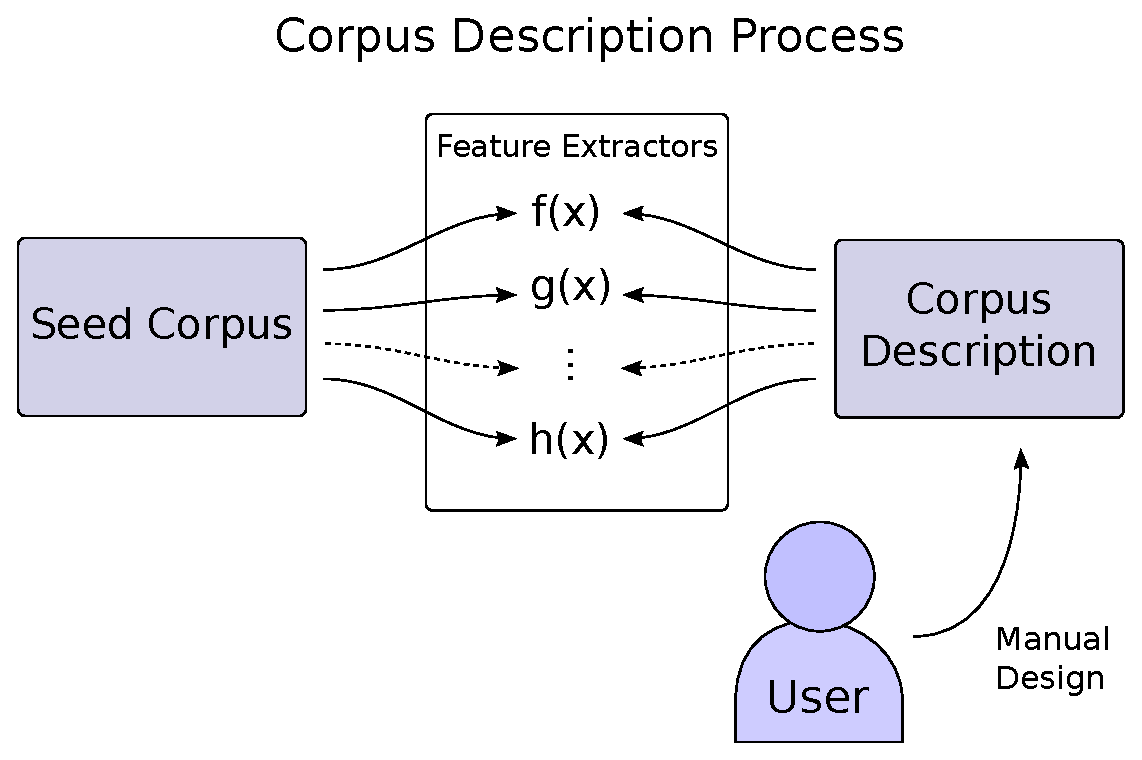
\includegraphics[width=0.8\textwidth]{rebuilding/profiling}
    \caption{Creation of a corpus description}
    \label{fig:rebuilding:profiling}
\end{figure}


The process of building a corpus description is outlined in~\ref{fig:rebuilding:profiling}.  For direct use, the user would specify their salient dimensions, and the distribution for each.  This is essentially a description of the sampling policy---where variables are discrete and nominal (such as genre labels), this would take the form of a table with desired proportions against each.  Where variables are continuous, a probability density function is defined.  Note that this method does not, without prohibitive complexity, allow for specification of interactions between variables\td{return to this and comment on it later}.

Profiling through the use of a `seed' corpus begins with specifications of the salient dimensions, the data for which are then read from the seed (by $f()$ and $g()$ functions in the figure).  As each document is read, the corpus description may contain information not only on marginal distributions for each variable, but also the effects of conditioning on one or more value.

Note that, whichever method is used, this stage is merely a metadata description task.  The corpus description document itself contains no more information than the metadata of the corpora from which is it built---indeed, where all variables are both external and nominal, this reduces to a simple table of frequencies for each desired value.  

Those specifying variables to describe must, as with all sampling, be mindful of their potential systematic correlations with variables of interest to any given research question.  The value of this approach is in documentation---it is possible for a researcher to eyeball the variables (and potentially their distributions) and determine whether or not a corpus is correctly conditioned for use inferring about a given variable.  This cannot be said for bootstrapping systems that use internal variables, which seek to copy corpus contents at the risk of varying their metadata.


% ---

\section{Retrieval}
Retrieval in accordance with the complex distributions specified in a corpus description is challenging in two ways:

\begin{itemize}
    \item Samples must be taken from the corpus description in accordance with a complex empirically-determined distribution;
    \item Any combination of variables sampled from the distribution must then be sought based on its metadata alone.
\end{itemize}

The former of these is difficult because many seed corpora may lack sufficient data to specify their distributions, and because of the high dimensionality of the distributions in question.  These issues may be addressed using techniques such as Gibbs, slice, or rejection sampling.  



\subsection{Resampling}

\td{cite this}
\begin{figure}[h]
    \centering
    \includegraphics[width=0.8\textwidth]{rebuilding/resampling}
    \caption{Resampling the corpus using MCMC methods}
    \label{fig:rebuilding:resampling}
\end{figure}



Resampling from the original corpus produces a `prototype' document, which has values of metadata fields that, over time, hold the same distribution as those in the seed corpus.  To perform this resampling, we must be able to sample from a distribution proportional to that of each variable conditional on all of the others, requiring that the corpus description contains information on interactions between values.

The process of constructing a new corpus is one of continually producing these `prototypes' conditional on the values of metadata already sampled, and then retrieving the text for each.  Resampling according to multivariate distributions is possible using Gibbs or slice sampling, both of which are MCMC techniques---the `output' distribution of prototype metadata will iteratively approach the distribution of input data.

This process is nonparametric, and thus able to accept arbitrary empirical input distributions and arbitrary modifications thereto.  This allows us to arbitrarily boost the sampling probability of a given category, or to ensure that variables with hitherto-unseen values are considered contributory to the output corpus.

Gibbs sampling is also commonly used to infer the posterior distribution of individual variables by fixing the values of the input distributions.  Though beyond the scope of this thesis, it would be possible to use this technique to fix input variables and identify the distribution of metadata values also described in the corpus description document.  This technique would be highly sensitive to the bias of the retrieval mechanism, and would require a particularly large seed corpus to operate meaningfully.


\til{
Theoretically speaking, the corpus is reconstructed as a distribution of all internal variables on the document, conditional on the values in the metadata.  So long as the retrieval engine can find documents fitting the distribution of input data, the output data will conform to the posterior distribution of word frequencies (or any other internal property one wishes to reason about).

Separation of the latent (internal) variables into a block is consistent with a 'block gibbs sampler'.  Ignoring them as a block is consistent with a 'collapsed gibbs sampler'.

% This is awesome: http://www.people.fas.harvard.edu/~plam/teaching/methods/mcmc/mcmc_print.pdf
}


\til{ Describe gibbs formally, and compare slice to it.  Describe the process of resampling from the output using the input distribution. }












\section{Method}


\section{Implementation}


\section{Limitations}





\chapter{Evaluation/Discussion}
\label{sec:evaluation}
%\section{Introduction}
\label{sec:evaluation:introduction}


We have seen in previous chapters (\td{which}) a number of scientific and practical issues that affect current corpus collection methods.

This chapter details the design and implementation of a method for performing number of common corpus building workflows.  These workflows are designed both as a continuation of the methods detailed in Chapter~\td{chapter 4} and as part of work with existing corpora, and represent areas of scientific importance in corpus studies.




The chapter begins in Section~\ref{sec:rebuilding:rationale} with an outline of the workflows involved, detailing the rationale behind each, and the value that formalising the process may yield.  Immediately following is an outline of the design of the method, specifying the processes involved and comparing them both to existing procedures and to the original workflows.

Section~\ref{sec:rebuilding:method} describes the mechanisms used to implement these designs, and covers the architecture of the software used to test the method.  It discusses the algorithms used, as well as the variables selected for the test system and the strengths and weaknesses of these as a mechanism for evaluating the method described earlier.  This section then specifies the technical details of the implementation, and provides details on the approximation and optimisation methods used.  

Finally, the conclusion relates the design and implementation of the method back to the aims detailed in \td{ref chapter 2}, drawing comparisons again to the capabilities of other existing systems.



\section{Evaluation Criteria}
\label{sec:evaluation:rqs}


The overall method used in this evaluation is one of treating the system to be tested as a method of replicating the features of a corpus, passing statistical properties of the input corpus through to the output.

The capacity of any system using auxiliary data to do this is dependent on the nature of the population, and how it relates to the input.  The data used for evaluation must then be a subset of the population of documents accessible using the search heuristics chosen---if testing with another seed corpus, one must change the search strategy modules to fit, changing the overall results of the tool.  Essentially, this is a manifestation of 'garbage in, garbage out': moving search strategies into the implementation merely makes this more explicit.

One method of testing this is to see the output corpus as a model of the input, given certain assumptions that include the selection of metadata types and search strategies: providing those assumptions hold, much of the variation in the input corpus ought to be explained by variation in the output.  Measuring deviance between the two allows us to identify specific areas of poor fit, which can then be improved either by altering the pluggable modules to fit the ground truth.

The purpose of this evaluation is to test both the search modules used for the particular corpora given, and the overall method: if no set of reasonable assumptions can be found, this is an indication either that the population of documents online is fundamentally different to that of the input corpora tested, or the method presented here is incapable \textsl{by design} of identifying appropriate documents.

% --

Research questions surrounding this method run to:

\begin{itemizeTitle}

    \item[Components] How valid are the assumptions of each of the retrieval methods and heuristics selected?

    \item[Overall Application] For general-purpose input corpora, to what extent (and in what manner) does the output corpus resemble the input `seed' corpus?

    \item[Feature Correlation] Do the differences between two input corpora match those between two corpora built using them as seeds?

    \item[Residual Variance] What consistent features remain variable between the output and input corpora, i.e. what data cannot be sought online using the heuristics/search methods selected.

\end{itemizeTitle}

The accuracy of each heuristic component is constributory to the excess dispersion in the output corpus.  By design these modules are unambitious, relying on existing methods and tools already tested in the literature, however, their performance upon the data used here will be evaluated in order to better explain sources of error.  As this system remains a proof of concept, the selection of these modules is limited.






\til{put in discussion: this restriction already exists for tools like bootcat, but without the explicit control over search mechanisms provided using the method being evaluated here.  Since there is no theoretical way around the `garbage in garbage out' problem, providing easy operationalisation to users is one approach to reducing overall methodological errors}

---notably, selecting a wildly different input corpus without changing the sources of data will result in wildly different 







\section{Performance of Heuristics}
\label{sec:evaluation:heuristics}
The heuristics selected for this evaluation are formed around Lee's BNC World index~\cite{lee2001genres}.  This selection was chosen because of their alignment to operationalisable, human-level metadata and the existence of multiple corpora with this level of annotation.



There are two main approaches to populating the corpus description using these heuristics: either read the seed corpus' contents and classify each data point, or read a list of metadata from an existing index.  The latter approach is used in this evaluation, since it is applicable to corpora with partially-missing data (such as the personal corpus data resulting from data gathering in Chapter~\ref{5}).

The accuracy of the classifiers listed here is responsible for minimising excess dispersion relative to the input corpus.  The nature of their residual error is also going to apply bias to the resulting data set.

Since many of these heuristics surround operationalising a corpus, a large body of research exists for classifying and extracting useful dimensions from texts.  The heuristics presented here are proof-of-concept only, and it is expected that the design of the heuristics used for a study is selected to match the theoretical basis of any analysis.

The heuristics presented here are document-level.  In most corpus designs, word count would be considered a measure of the size of the corpus (rather than a property of its constituents).  The method evaluated here is capable of retrieving truly IID samples at different levels, and demands a different selection of heuristics and metadata when operating at the word or sentence level.  Document level metadata are both high-level enough to be distributed for confidential corpora and descriptive enough to enable accurate retrieval (by contrast, word or part-of-speech frequencies would reveal much of the contents of the original corpus, which may not be desirable).

\subsection{Audience Level}
* Reading level used as an estimator
* Means, standard deviations computed from BNC
* Accuracy test with nearest-mean classifier

\subsection{Word Count}
* Compare word counts to BNC files
* Talk about boilerplate removal

\subsection{Genre}
* Classifier description
* Talk about rationality of errors
* Talk about how difficult this is
* Evaluate unigram, ngram, naive bayes
* Comment on the choice of genres, how artificial or simple ones might be better (perhaps aligned with data source such as DMOZ?)





\section{Performance of Resampling}
\label{sec:evaluation:resampler}

The accuracy of the resampling process depends lagely on two user-controlled properties:

\begin{itemize}
    \item The amount of smoothing applied to continuous metadata in the corpus.  Since values are selected from the smoothed corpus values, it is possible to select values that are non-identical to the input corpus.  This is generally a desirable property, and the kernel function used to smooth the input data is user-defined and has known statistical properties.
    \item The number of documents selected.  As this increases, the overall distribution of the output corpus converges to that of the corpus description file.
\end{itemize}


The intricacy of the input distribution largely defines the necessary size of the input corpus: an input corpus that is defined only in terms of simple marginal distributions is simpler to reproduce, that is it contains \textit{less information}, than one built using the full conditional distribution of a large, general corpus such as the BNC.

The question of when to stop sampling documents is related to the problem of corpus size in general: the output corpus is conceptually a model of the input corpus, and should contain enough data to be representative of the relationships therein whilst following the same guide.  This is best assessed by measuring the uniformity of residuals.  A suitable end condition for many uses of the output would thus be a combination of corpus size and residual uniformity (notably it is possible to constantly balance the uniformity of residuals during the rejection sampling phase too).

The evaluation here establishes the resampling algorithms' ability to produce copies of the input corpus with uniform residuals, and establishes a 'best case' baseline against which the results of document retrieval may be compared.

The research questions answered by the analysis here run to:

\begin{enumerate}
    \item Does the resampler converge on the same distribution as its input?
    \item How many `target' documents are required to converge upon the input distribution (at some known probability)
\end{enumerate}


\subsection{Method}
Evaluation of the selection method is possible separately to document retrieval as the input distribution is known.  This means that, unlike a bootstrapping operation, we can rely on model deviance measures (rather than heuristics such as autocorrelation) to indicate the point at which we have sufficient data to represent the input distribution.  Since documents are retrieved and compared against their `target' as selected by this process, it is thus possible to guarantee conformance to some property of the input distribution, providing retrieval is performed accurately.  The eventual error for the corpus is a sum of these two deviances.


\begin{figure}[Ht]
    \centering
    \includegraphics[width=0.9\textwidth]{evaluation/resample-overview}
    \caption{Data flow for evaluation of the sampler.}
    \label{fig:evaluation:resampling:overview}
\end{figure}


The data flow outlined in Figure~\ref{fig:evaluation:resampling:overview} is identical to that used for the final selection, with the omission of a retrieval stage at \textsl{\color{red} x}.  This means the evaluation will be performed under the assumption that the retrieval process is always able to find a suitable document.  The operation performed by the evaluator is essentially a comparison between two distributions, and may be performed using any number of algorithms with the one requirement being that it can practically be executed after each document is retrieved (note that for the purposes of this evaluation, such a requirement is less critical).

Evaluation methods provided in the prototype implementation are:

\begin{itemizeTitle}

    \item[Mean Error] For each dimension, the sum of the deviance from each document to its target value is divided by the number of documents in the collection.  This provides an asymmetric form of the commonly-used Mean Squared Error.
    \item[Distribution Comparison] A commonly used method for comparing empirical distributions, this is computed by taking the differences between the cumulative density of each dimension's data and is thus less sensitive to order than MSE methods.  Typically these methods are able to provide confidence bounds related to statistical significance.
    \item[Linear Modelling] A linear model is constructed and fit with parameters according to the input dimensions.  If this model proves statistically equivalent to the null model, then the residuals are considered uniform.

\end{itemizeTitle}


For the purposes of this evaluation, a distribution comparison method, Log-likelihood, was selected due to its known statistical bounds and wide use in corpus linguistics\footnote{It it worth noting that the log-likelihood statistic is just one of a large number of valid goodness-of-fit tests, the main contender being two-sample Kolmogorov-Smirnov}.  The major disadvantage of using this method, that it is harder to directly relate to the content of each text, is not relevant at this stage of analysis.


Log likelihood comparison methods are already widely used in corpus linguistics for keywording and corpus comparison, and have the notable property of measuring significance (using Wilks' theorem), rather than effect size (as with many information-theory-based deviance measures such as MI and Jaccard).  This evaluation makes use of such properties in that we desire to know at what point the output distribution is, to a given standard of probability, the same as the input: as we do not control the size of the input distribution we are unable to control the ultimate power of the test and thus the effect size.

This comparison of the output and input distributions was repeated as documents are re-sampled, the point at which the two cease to be significantly different noted.  This process should establish both RQs:

\begin{enumerate}
    \item Load input corpus;
    \item Repeatedly sample from the input corpus, inserting documents into the output corpus;
    \item After each document, compare the output distribution to the input.
\end{enumerate}


Note that this method treats each metadata dimension of the input corpus as an independent distribution, effectively evaluating the joint distribution of the sample.  This was done to permit comparison where obtaining a sample large enough to provide sufficient statistical power is largely impossible --- even in the BNC, there are seldom many documents that share \textsl{all} metadata values.  This has the effect of weakening the test such that the `Conditional' sampler is indistinguishable from the `Marginal' sampler (as mentioned in Section~\ref{sec:rebuilding:method:retrieval:resampling}).



\subsection{Results}

The evaluation here focuses on categorical values with over five members due to the asymptotic nature of the log-likelihood statistic making it unreliable below this number.  As such, we bin the word count into 17 bins, and use the true BNC readability category rather than the (continuous) Fleisch reading ease score.  This results in three variables that must converge prior to similarity being determined:

\begin{itemizeTitle}
    \item[Genre]  The genre category, as fit using the classifier heuristic mentioned elsewhere, only using all 70 categories;
    \item[Words]  The word count, binned to form bins with no fewer than five texts in each;
    \item[AudLvl] Audience level, categorised as `high', `med', and `low';
    \item[Mode]   \textbf{S}poken or \textbf{W}ritten.
\end{itemizeTitle}

The word count is binned irregularly due to the low frequency of files with more than 80,000 words listed in the index.  This results in a distribution shown by the historgram in Figure~\ref{fig:evaluation:resampling:bncwordhist}, with the minimum bin frequency being 8.  Other variables were left unmodified.


\begin{figure}[Ht]
    \centering
    \includegraphics[width=1\textwidth]{evaluation/4waybnchist}
    \caption{Word count distribution from the BNC index (n=4054, breaks at 5k < 80k, max=428248)}
    \label{fig:evaluation:resampling:bncwordhist}
\end{figure}


The convergeance rate of each of the variables is, as mentioned above, dependent on the information content of the input bins' frequencies (due to the complexity of the sample) and the number of bins with fewer than five members (due to log-likelihood converging slowly to the $\chi^2$ distribution).  Each variable's convergeance may thus be appropriately expressed in terms of how long the average bootstrapping process takes to converge upon the distribution to a given confidence value, relative to the size of the input.

A basic description of the bins used for each input metadata item is presented in Table~\ref{table:evaluation:resampling:inputdist}.  Medians and interquartile ranges were used as centrality and deviance measures due to the Zipfian nature of the bin distributions (a feature expected to manifest in most corpora).  The `ID' column gives the `index of dispersion' --- a normalised measure of the variability in the distribution's bins computed by dividing the centrality measure (median) by the centrality measure (median).

% TODO: table with variable, bin count, num<10, stdev, mean, convergeance mean, convergeance confint@95%
\begin{table}[Ht]
    \centering

    \begin{tabular}{ |l|c|c|c|c|c| }
        \hline
        Metadata & bins & $|n_{bin} < 10|$ & $median(n_{bin})$ & $IQR(n_{bin})$ & ID  \\
        \hline
        Genre & 71  & 16 (22.5\%)   & 26    & 49        & 1.88    \\
        Words & 18  & 2 (11.1\%)    & 117.5 & 359.25    & 3.05    \\
        AudLvl& 4   & 0 (0\%)       & 869   & 317.5     & 0.36    \\
        Mode  & 2   & 0 (0\%)       & 2027  & 1117      & 0.55    \\
        \hline
    \end{tabular}
    \caption{Distributions of metadata dimensions in the input corpus (BNC index)}
    \label{table:evaluation:resampling:inputdist}
\end{table}

The figures in Table~\ref{table:evaluation:resampling:inputdist} represent common cases for real-world corpora:

\begin{itemize}
    \item `Mode' is a simple binary classification with very different group sizes.
    \item `AudLvl' is a simple classification with a very `flat' distribution.
    \item `Words' is a bimodally distributed measure with a large amount of variation but also very large numbers in each bin.  This is a good representation of the counts of many linguistic features.
    \item `Genre' is moderately heterogenous, yet has a distribution with many low-frequency items in it.
\end{itemize}

We may reason from the index of dispersion that convergeance will occur faster for `AudLvl' and `Mode' than for `Genre' and `Words' --- the ordering of the other two largely being determined by the conservative estimation of log-likelihood for low-frequency bins.


\begin{figure}[Ht]
    % ./analysis/loglik-significance.r
    \centering
    \includegraphics[width=1\textwidth]{evaluation/4wayCI95}
    \caption{Log-likelihood scores and 95\% confidence intervals for each metadata property during resampling (100 repetitions of 100,000 documents)}
    \label{fig:evaluation:resampling:4wayCI95}
\end{figure}


Figure~\ref{fig:evaluation:resampling:4wayCI95} displays the log-likelihood score of the output distribution as it is built.  These graphs clearly illustrate the relative complexity of the input distributions, as well as the downsides of estimating log-likelihood measures for low-frequency results.  After an initial burn-in period (the end of which is marked when the output distribution size matches that of the input), all dimensions gradually converge upon the target distribution.  For any input distribution with low counts, the similarity measure will not be accurate until these lowest bins are filled---marked on the graph roughly as the point where the output distribution is equal in size to the input.%\td{though this is not entirely precise and I think is estimable using binomial}.

The two simpler distributions, `Mode' and 'AudLvl', peak at levels well below the 95\% threshold chosen for the log-likelihood statistic.  In the case where the `target' input distribution is defined by profiling an existing corpus, this implies that we could properly build a corpus \textit{smaller} than the input (though unfortunately this is not rigorous without also know the relationship of the original input corpus to the population as it is itself generated from that sample).  The relatively confident estimates for these parameters at a 1:1 input:output ratio backs up the rational expectation that large numbers of documents in few bins will be easy to replicate.

A marginally more complex distribution of metadata in the form of the `Words' dimension shows, again, fast convergeance, requiring an output distribution roughly twice the output to replicate with 97.5\% confidence.

By far the most complex input data, `Genre', takes much longer to converge, requiring a ratio of roughly 12:1.  This result is largely a function of the low bin frequencies and the large proportion of bins that have values below the threshold at which log-likelihood may be relied upon to provide a moderately-conservative estimate.

The speed of convergeance reflects the variability that is permitted in any subsequent retrieval process: fixing the `Mode', for example, will lead to a corpus with known proportions of spoken and written text, but variability otherwise according to the population from which they are sourced.  If a particularly large corpus is available with a desirable sample design, restricting only one dimension merely refines the original sample\footnote{Of course, such a situation is difficult if the corpus from which documents are not tagged with relevant metadata, something unlikely if that dimension was not already in the sample design}.

\paragraph{}

The process of random resampling detailed here is in many ways uninteresting: after all, the experiment detailed above merely selects items based upon existing metadata.  The value in the above technique lies in its mode of use:

\begin{itemize}
    \item The distribution converged upon is arbitrary, and may be defined in the absence of an input corpus (or as a modification thereof).  This allows relaxation of a corpus description's requirements to reduce the necessary oversampling ratio above, or the addition of specific metadata items where the source of documents is particularly easy to sample according to certain properties.
    \item Halting the resampling process at any stage, due to the random selection method used, leads to an unbiased output corpus (though it may well be imprecise to the point of irrelevance).
    \item After resampling of candidate documents through a process of resampling (which has known bounds of error), the process of retrieving documents can be compared against a gold standard.
    \item When starting with a manually-designed corpus (which has bin sizes only relevant to one another), convergeance can only be achieved where the output corpus size is greater than or equal to that of the input corpus.  Aside from fitting issues where bin sizes are small, corpora fit using the same distribution shape should converge at the same size (i.e. \textsl{not} relative to the input corpus size).

\end{itemize}


% TODO: Experiment on convergion point by input n, and/or autocorrelation
% linear models for each, comment on confidence



% ---------









% \til{integrate the below better, it was written standalone.}


The relationship described by the log-likelihood scores of the two corpora describes the confidence one may have in the original, input, corpus: an input corpus with very few documents in each `bin' is less powerful when used to answer questions using data in that bin, and so will require a greater number of documents in the output corpus to achieve confidence at the same effect size.  This is a useful heuristic, as it ensures that samples are never output that are not in some way large enough to be confident about their distribution, thus enforcing a minimum sample size.  Unfortunately, if this comparison is based on duplication of an existing sample (such as in this case) such an adjustment is non-rigorous as it is based upon the sample parameters, which have an unknown relationship to the population parameters they estimate.  Essentially, whilst this is a heuristic indicating internal validity, it does not ensure external validity.

A notable property of the resampler is that, even if the confidence of the output corpus being 'converged' to a given confidence level is very low (i.e. the log-likelihood score is above a given threshold), the output corpus is unbiased relative to its input due to random selection.  In addition, the convergeance of a corpus with a simpler design than the source corpus will occur at a number of documents lower than that of the input corpus, making it possible to resample an existing corpus using a design with \textit{simpler} metadata properties.  In this case, the `simplicity' of the design is defined by the information in the design distribution relative to the information content of the source corpus.  For example, if our experiment did not care about genre, it would be possible to sample texts directly from word count and audience level, producing a corpus with fewer texts yet the same coverage of those two dimensions.
%a mere \td{n} nexts in with a \td{n\%} confidence of representing the input corpus.






\begin{lstlisting}[language=,caption={Example output showing the recursive resampling process.},label=lst:evaluation:resampling:resampleexample]
example of running the thing:

Loading profile...
[genre] Loading classifier data from memdump: ./resources/list_classifier_dump.dat...
Loading corpus from /tmp/test.corpus...
Building sampler for corpus #<Corpus:3:269543840>...
Using full conditional sampling with Z = 1.645, sd = 30
Creating (virtual) output corpus...
Corpus created using 3 dimensions of metadata:
  - GENRE of type #<Impute::DiscreteDistribution:0x000000025d2710>
  - Word Total of type #<Impute::SmoothedGaussianDistribution:0x000000025d26c0>
  - Aud Level of type #<Impute::DiscreteDistribution:0x000000025d2648>
Selecting random document from #<Corpus:3:269543840>...
 - dims: 3, docs: 4054
 - dims: 2, docs: 4 (Word Total == 32528.538691473)
 - dims: 1, docs: 1 (Aud Level == low)
=> #<Impute::Document:0x0000002123f3b8
 @dimensions={"Word Total"=>32528.538691473, "Aud Level"=>"low", "GENRE"=>"W_pop_lore"},
 @id="115f72d0-94cc-4c4d-91d1-6b8cbe18a081",
 @meta={},
 @text="">
\end{lstlisting}







\section{Performance of Retriever}
\label{sec:evaluation:retrieval}
\subsection{Method}
\label{sec:evaluation:method}
Discuss the evaluation methods.  Firstly talk about the error monitoring methods built into the program, then detail the linguistic feature analysis.  This is the main body of the analysis of the method and doesn't cover the heuristics


\subsection{Data}
\label{sec:evaluation:method}
Discuss which corpora were chosen and why

\subsection{Results}
\label{sec:evaluation:}
Provide quantitative measures for the two evaluation methods
%#\subsubsection{Partial/white box}
%Show how well classifiers and heuristics behave
\subsubsection{Complete/black box}
Show how well the whole system works




\section{Discussion}
\label{sec:evaluation:discussion}




The evaluation above is a white-box exploration of the characteristics of each component in a context similar to many real-world demands.  It displays variable performance.

Firstly, the performance of classifiers when operating on text must be established relative to the research question.  In this case, that was particularly tricky for a number of practical reasons which shadow the classical manual corpus construction issues:

\begin{itemize}
    \item Linear separability of dimensions such as readability was insufficient to create a classifier with good precision/recall scores.
    \item The complexity of some sampling criteria requires the use of black-box models that are themselves unpredictable, and require training using auxiliary data.
\end{itemize}

Both of these are common cases when dealing with `human', research-aligned sampling criteria, and both are rightly recognised as key areas for improvement in text processing.  The deficiencies in real-world performance of this classification process must be assessed on a case-by-case basis: for certain sampling criteria, classification is made trivial by the existence of metadata (for example the recipient fields in emails) or existing mechanisms online for directed retrieval.  

This limited classification capacity comes with a silver lining, however: unlike other bootstrapping approaches, it is possible to separate and independently evaluate the performance of any classifier used.  In turn this makes it possible to re-use others' research in this area and make incremental improvements over time.  Secondly, classification accuracy is improved by application to well-specified problems of limited scope: a priority that aligns well with the core values of a good sampling scheme.


Examination of the BNC categories used here also reveals the loose nature of classification therein: many categories are defined according to fairly fluid concepts of varying specificity, and many overlap significantly.  This is evidenced by the relative performance of classifiers built with minor changes to their classes, and by the keywords used by the Bayesian models.  


% -- 
\paragraph{}

The bootstrapping process, separated into a process of building a prototype corpus, has been shown to converge within a timeframe that is compatible with automated retrieval.

For the BNC example outlined here, roughly $12$ times the input corpus size is required to converge with 95\% confidence.  This is an impediment to use of these techniques, except where:

\begin{itemize}
    \item The input corpus is fairly small and low-variance, such as in the case of special-purpose corpora;
    \item Retrieval of documents is automatic and fast.
\end{itemize}

The former of these weakens any requirement for the latter and vice versa: the example presented here is an example of speeding up retrieval to allow for large-scale corpora, something that places particular focus on the quality of the retrieval process.

\til{Unfortunately, retrieval is the dodgiest bit :-(}

% --
\paragraph{}

Automated retrieval is the part of the method with the greatest number of practical challenges. The method used here is deliberately comparable to the bootstrapping approach used by BootCaT\td{cite?}, in part to use the prototype corpus approach for an evaluation of search engine retrieval methods.

The evaluation here focuses on genre-based retrieval.  This is of particular salience to many linguistic research questions, and is well aligned to search engine indexing behaviour --- an ideal automated retriever would go far beyond this to use document metadata and different sources of text (such as academic repositories).

Keyword-based search engine retrieval is shown, in the case of the BNC, to have roughly central error --- this is encouraging, though it is unclear how well this holds for other corpora.  Of particular interest is the application of the method to special-purpose corpora, which are (by design) strongly biased.

Of greater concern is the systematic over-representation online of certain genres.  This implies that automated retrieval must advance significantly in order to sample many corpus designs, or that it must be complemented by manual methods where documents are difficult to locate.  The exact thresholds of `difficulty' there must be determined on operational grounds of cost and time --- for large-scale corpus building operations, a largely manual approach may be the best method of ensuring quality whilst still leveraging the benefits of the quantitative profiling and resampling approaches.



% --
% \paragraph{}


\til{Compare more to RQs...}
\noindent\makebox[\linewidth]{\rule{\paperwidth}{0.4pt}}






 % ---
%
%
% The performance of each component within the system is, as we have seen above, variable.  For certain classes of corpus, such as those originating from web data themselves, replication and rebuilding promise to be relatively straight-forward and easily automated.  For corpora such as the BNC, however, a number of practical issues are particularly difficult to dodge.




\subsection{Future Work}

There are a number of areas with clear opportunities for future work.

Firstly, heuristics must be sought that are able to properly classify variables of interest.  These already exist due to great utility in other areas, and their properties are well understood.  Nonetheless, some may require modification or further study until proven useful for a particular corpus building task.

Much further work is also possible evaluating the resampling process, and producing estimates of required sample size.  This will never form an authoritative guide to sample size due to the lack of knowledge about experimental power and the dependence on the `seed' corpus, however, it may act as a guideline for corpus builders.

Finally, the retrieval process must be improved significantly if it is to be an acceptable alternative to manual construction.  Since error is known for each document returned, it is likely that search-based retrieval can be improved significantly by better targeting of search terms and document sources.  One promising avenue here would be hybrid retrieval: using automated means to gather most documents and then passing difficult-to-find terms and criteria to a person for manual additions.

Additionally, the utility of the method when applied to different sample designs is of particular importance: when analysing the corpus using a bag-of-words model, for example, one would be able to sample only individual words from the web.


% Link to an appendix with the generalised form of the proxy corpus thingy?
% Cover the heuristics and modules that need making, and possible tweaks to the error feedback mechanism.  Also comment on the knowledge we have of various populations online and how this impacts inherited bias.






% Talk about the various strengths/weaknesses w.r.t. the original RQs and the goals in ch5.
% \subsection{Choice of submodules}
% talk about which heuristics seem good, and what needs improving


\section{Summary}
\label{sec:evaluation:summary}

Conventional corpus sampling techniques are, fundamentally, based on those used elsewhere.  There is, however, much confusion on the topic, and unwarranted debate over whether or not corpora are comparable to typical samples.

Much of this debate has stemmed from tradition, being sparked by the complexity of corpus designs such as Brown's, which relied heavily on expert opinion and inclusion of text according to a deliberately non-representative policy.  Much of this subjectivity is, in reality, a reaction to practical challenges that faced the first corpus construction efforts.

Many of these practical challenges have either changed in nature, or been solved.  Digitisation and POS tagging are now largely automatic affairs, and documents for inclusion are often born digital.  For UK researchers, there is even relief from a number of intellectual property issues.

Unfortunately, however, some have proven harder to solve.  There are still large challenges to the problems of population definition, and definition of a widely-agreed-upon taxonomy for genre definition.  Additionally, access to documents, even where technically possible, is often restricted by private corporations, or filtered through systems such as search engines that act as black boxes.

These remaining challenges are still limiting the corpus building process, and prevent the use of the most quantitative random sampling techniques.  Even those that are part expert-informed, such as stratified sampling or cluster sampling, require widespread agreement on taxonomy selection.  It is unlikely that there will be any one answer to such theoretical issues, as these must be defined relative to the research question.

The Web-as-Corpus movement offers a democratisation of the corpus building process by easing a number of the retrieval and enumeration problems.  These come with a significant challenge of their own, however, in that each user must then perform all of the stages of a corpus construction effort: from unambiguously specifying population parameters to cleaning and preparing the data.

This process can, at least, be automated.  In so doing, it is possible for researchers to vary their corpus designs and tailor them to meet individual needs.  For this to occur, tools and methods must be produced that are able to take design goals and, without significant further effort, produce corpora from them.

The role of this thesis is to explore this space, investigating corpus sampling and identifying areas where WaC approaches may mitigate remaining issues.  The ultimate goal is to provide methods and tools which allow users to rationalise and operationalise design criteria to produce their own valid and useful corpora.







\chapter{Conclusions \& Review}

% Summary

This thesis has examined the problem of improving corpus sampling from a number of perspectives.  This chapter will serve to summarise these, before offering an overview of significant areas for further research.

Chapter~\ref{sec:longitudinal} presents a motivating study of link rot in open-source corpora, finding large variations in document half-life using a URL-seeking method.  This illustrates that temporal effects have a significant impact on the availability of data, and that such effects vary according to source.  Much literature exists that has related these to layout features (such as the role of navigation and landing pages), yet the impact this has upon linguistic content is less well understood.

In order to make such investigation possible, a cohort sampling approach is necessary, performed at a high resolution over a long period of time.  The LWAC tool automates this process, providing a mechanism to construct large-scale corpora that are indexed by time as well as URL.  Key to the utility of such a tool is its performance, which was shown to be adequate to construct corpora in the millions of documents, sampled daily.

This wealth of data enables analysis not only of `simple' availability, but also changes through time due to editorial processes or site redesigns.  This may allow sociolinguistic analysis surrounding specific events, or a more general picture of long-term language change through time.  It is hoped that the latter of these can be used as auxiliary data to inform stratification of future general-purpose corpora (or at least their web-based components).

% ---
Chapter~\ref{sec:personal} presents a case study detailing a short-term linguistic census of a single subject.  The sample design used therein is a `narrow and deep' design, orthogonal to the 'broad but shallow' coverage of the large national corpora.  This makes it particularly useful for judging rationally how well such data apply to individuals, and offers a way to retrieve metadata not found using conventional data gathering methods.

Such a detailed sample also provides a mechanism for reasoning about problems of corpus size: the data observed in just two weeks for a single subject yielded almost a million words.  Assuming significant inter-person variation for a given linguistic feature, this implies that a population of ~60 million people cannot be well represented by a corpus of just a few million words.  Quantitative knowledge of inter-person variation is needed to operationalise this, but such data could be gathered using some of the automation methods presented.

Such methods were largely taken from lifelogging, a field chosen due to its focus on unobtrusive, best-effort, and wide-ranging sampling techniques.  These proved to be significantly more troublesome than expected: though automation was assistive, much manual correction was necessary to operationalise the data, including the need for a human-interest model to correct summary statistics that were gathered at a low resolution.


% ---
Chapters~\ref{sec:rebuilding} and~\ref{sec:evaluation} cover a method for `profiling' a corpus purely based on independent variable specification.  This profile has many potential uses, both as human documentation for a corpus and as a machine-readable descriptor, and constitutes a way to gradually refine corpus designs over time.

This system is one designed to extend and generalise the approach taken by BootCaT in order to make its selection criteria easier to operationalise.  It is designed to be modular, allowing those building a corpus to re-use algorithms and taxonomies in a simple manner: essentially, the aim is that the tool should be working using the same concepts and distinctions as the desired sample design.

Monte Carlo techniques were used as a method for operationalising the profile, something that was shown to achieve convergence to the desired distribution within a tractable period for a BNC-like corpus of written text.  The classifiers required to identify documents for final selection were shown to be workable, but their performance was borderline for the more complex dimensions such as genre---this is in part due to the ambiguity in the test data's taxonomy, and in part due to the difficulty of large-scale classification tasks.  Such issues are of wide utility, however, implying that improvement in this area will not require specific study.

Retrieval of documents according to the prototypes was shown to be possibly the biggest challenge.  This is in part due to the classic corpus sampling problems of being unable to locate documents in a uniform and reliable manner, and in part due to the biases seen online.  A number of methods were presented to work around these issues, such as manual selection or use of manually-curated web indices, and evaluation of these remains as further work.




% --------
\paragraph{}
To revisit the problem of representativeness, this thesis has taken the view that any such question must be framed in terms of a larger study design.  This is not to say that general-purpose corpora are impossible to create: sampling larger populations is such a challenging and resource-intensive endeavour that it will most likely always have to be offloaded onto a third party.

The aim, then, is to provide a general-purpose corpus that is uniformly representative for a wide, and well-specified, set of research questions.  This corpus should be sampled using random sampling techniques, and this thesis' tools have been designed to inform stratification efforts with this in mind.  Such a corpus should also be unambiguously and comprehensively documented: assumptions should be made explicit in corpus documentation so that they may be compared against those made by researchers, and the limitations of the intended use of a corpus should be stated in quantitative terms.

The contributions within this thesis have been targeted to provide some insight into the underlying population that is not possible using current techniques.  I do not suppose that these alternative sampling designs will be used in their own right (though there is utility in this for some), but that the perspective they yield may be used to inform and improve upon existing corpus retrieval methods.


% Kilgarriff \& Grefenstette's issue with web corpora\cite[p. 343]{kilgarriff2003introduction}:

% \begin{quote}
% The Web is not representative of anything else. But neither are other corpora, in any well-understood sense.
% \end{quote}












% Further Work
\section{Further Work}
As much of this thesis has been exploratory, there is a wealth of further work necessary to maximise the value therein.  Whereas each chapter contains numerous notes in context, this is a high-level summary of the major avenues of inquiry.


% ====================================================================================
% \subsection{Further Work}
% Currently, workers in LWAC do not evaluate JavaScript or build a DOM (though they do send and receive cookies) --- increasingly these features are used by websites to display content, and extending workers to handle them broadens the set of pages it's possible to retrieve meaningfully.  Such an extension is expected to incur a heavy performance penalty, however, as it massively increases the work done by each client during downloads, and complicates the resulting data.

% The field of survival analysis offers a large number of techniques for studying the change in a cohort over time, however, this is largely focused on the existence of simple regressor variables.  This is suitable for technical properties such as those focused on by search engine designers, but less approproiate for digesting large quantities of text.  Techniques for time-series analysis of large corpora are developing, but are usually not based around a cohort-based design.

% The distributed nature of LWAC makes it possible to study geographical effects --- this is something that would require only modest outlay as virtualised infrastructure becomes cheaper.


% Further sampling and analysis is necessary to confirm the issues highlighted above.  This paper comprises a preliminary look at data sampled in a longitudinal study, which will go on to relate the influences of extrinsic document features (which may be used to inform sampling strategies) to their linguistic content.  

% This will involve, primarily, identifying the extent to which document attrition applies bias on linguistic content, rather than technical features, and how this varies through the sampling period.  Issues of particular interest include:

%





\subsection{Large-Scale Longitudinal Document Attrition Studies}
A large-scale longitudinal sample of WaC sources is one obvious extension to the work in Chapter~\ref{sec:longitudinal}\footnote{Indeed, one was underway, but due to technical failures the results were not ready for publication here.}.

Such a study would be able to answer questions not only on the rate of decay (as has been addressed elsewhere), but also the shape of the decay curve, hitherto presumed to be exponential for most types of data.

Further to this, there are many web page changes that do not constitute `link rot' in that the original information may still be present, but are still interesting for various linguistic and social questions, for example how often documents are changed in response to news events, or have their boilerplate changed in order to affect the context in which documents are presented.

Ultimately, developing a linguistic understanding of change through time will require significant work, however, a single large sample could provide useful information to those seeking to use large existing web or monitor corpora.

\subsection{LWAC Distribution}
LWAC's distributed design lends it particular powers in distinguishing web access issues from a geographical perspective.  With the low price of virtual machine rent, a network of LWAC clients could easily be constructed to access a number of websites from differing locations.

Such a configuration would reveal geographical changes made by site administrators for reasons of editorial control, censorship, and interference by service providers (Phorm\cite{clayton2008phorm}, for example).  This would open an avenue for investigation of a number of social factors, particularly as the (time-series) results could be compared and correlated with many real-world regressors, such as the incidence of political events.  Such approaches are already being widely used in social media analysis\cite{achrekar2011predicting,bollen2011twitter}, though the high number of societal covariates renders such studies difficult to validate.

\subsection{Slimmed-down Personal Corpora}
A natural progression of the work in Chapter~\ref{sec:personal} is the repetition with more subjects.  This is troublesome in part due to the in-depth coverage of language sampled, something that is likely to be less than critical for many research questions (such as those primarily concerned with `standard' day-to-day interactions, or even simply those using a computer).

There are many mechanisms which could be used to establish a provisional model of demographic linguistic variation based on partial sampling of each subject, perhaps elective using smartphone technology, down to the level of questionnaires.  This dataset could be added to gradually, and used to guide large diachronic sampling efforts as a form of auxiliary data.

This would require work to formalise and proceduralise the data gathering methods presented, in order to discount those with the least `effort efficiency' and maximise automation.  The continuing ubiquity of smartphone technology offers a vehicle through which to distribute such methods and collect resulting data.

Operationalising the results of such sampling is also an open question, though such work would largely require the application of existing stratification and re-weighting techniques.  This would allow an experimenter to select a small sample demographic, and then use a general-purpose corpus to augment it with larger quantities of linguistic information in a representative manner.  In order for these methods to be useful at a large scale, they should be informed by further work on power analysis, which is currently in its infancy in corpus linguistics.



\subsection{Improved ImputeCaT Modules}
The performance of the ImputeCaT corpus profile retrieval tool is currently constrained primarily by two factors:

\begin{itemize}
    \item The accuracy of classifiers used to identify document distributions and class membership during profile generation and candidate document selection;
    \item The specificity of retrieval methods.
\end{itemize}

The former of these is the subject of much ongoing research, and can be expected to progress gradually due to its utility in many areas.  The design of ImputeCaT is such that this may be leveraged easily to provide continuing accuracy improvements.

The latter is more challenging: though ultimately corpora can be retrieved manually (incurring only the error seen in inter-annotator scores for a given taxonomy\cite{sharoffs2015}), the scalability of automated corpus construction is born largely of its ability to retrieve documents online in an unsupervised manner.  This is currently limited by the search-engine-based retrieval mechanism demonstrated here.

Many options exist for this, such as the use of web directories, supercorpora, semi-supervised topic modelling, or crowdsourcing.  Each of these should be evaluated relative to typical corpus construction tasks in order to determine its suitability for given study designs: indeed, it is likely that some exhibit biases such that they are unable to replicate some samples.


\subsection{Bias Estimation}
Finally, the convergeance-based design of profile-guided retrieval offers the first few avenues through which to explore the bias of sources.  Currently, bias in retrieval methods is conflated with classification error, something that is also far from negligable.

The approach of seeking a series of known document properties, however, leads to the obvious method of simply measuring how `difficult'\footnote{Ideally measuring difficulty for a typical human.} it is to retrieve a document given certain parameters.  Differences between this difficulty-of-retrieval metric and an equivalent measured based on human performance should yield biases in online sources.

Such a measure would be highly dependent on many unstable variables, however, such as the retrieval methods used, sample design, and temporal/contextual factors.  Nonetheless, this offers a real-world take on representativeness without reliance on variance and homogeniety measures.

As ever, these methods are dependent upon finding a human analogue task that acts as a well-agreed-upon baseline: ultimately, without such a research question, the question of representativeness is unanswerable.




\begin{center}
\vfill
{\fontfamily{pzc}\selectfont C'est fini!}
\vfill
\end{center}






% =============================================================================
%  Bibliography
% =============================================================================
\pagebreak%
\bibliographystyle{swBibStyle}%
\backmatter%
\bibliography{../bib/PhilScience,../bib/CorpusDesign,../bib/Representativeness,../bib/Sampling,../bib/PersonalCorpora,../bib/WebAsCorpus,../bib/Methods,../bib/DocAttrLREC,../bib/DownloadTools}
% }


% =============================================================================
%  Auxiliary stuff
% =============================================================================
\pagebreak
\appendix
\addcontentsline{toc}{chapter}{Appendices}
\renewcommand{\thesubsection}{\Alph{subsection}}
\pagenumbering{Roman}


% =============================================================================
%  Appendices 
% =============================================================================



\chapter{Lee's BNC Genres}
\label{sec:appx:sample}
Lee's BNC genres go here, in a table probably.  'two do'





% =============================================================================
%  Fin.
% =============================================================================
\end{document}
